\documentclass[a4paper, 10pt]{article}
\usepackage[utf8]{inputenc}
\usepackage{verbatim}
\usepackage{listings}
\usepackage{graphicx}
\usepackage{a4wide}
\usepackage{color}
\usepackage{amsmath}
\usepackage{amssymb}
\usepackage[dvips]{epsfig}
\usepackage[toc,page]{appendix}
\usepackage[T1]{fontenc}
\usepackage{cite} % [2,3,4] --> [2--4]
\usepackage{shadow}
\usepackage{hyperref}
\usepackage{titling}
\usepackage{marvosym }
\usepackage{subcaption}
\usepackage[noabbrev]{cleveref}

\usepackage{tikz}
\usetikzlibrary{arrows}

\renewcommand{\topfraction}{.85}
\renewcommand{\bottomfraction}{.7}
\renewcommand{\textfraction}{.15}
\renewcommand{\floatpagefraction}{.66}
\renewcommand{\dbltopfraction}{.66}
\renewcommand{\dblfloatpagefraction}{.66}
\setcounter{topnumber}{9}
\setcounter{bottomnumber}{9}
\setcounter{totalnumber}{20}
\setcounter{dbltopnumber}{9}


\setlength{\droptitle}{-10em}   % This is your set screw

\setcounter{tocdepth}{2}

\lstset{language=c++}
\lstset{alsolanguage=[90]Fortran}
\lstset{basicstyle=\small}
\lstset{backgroundcolor=\color{white}}
\lstset{frame=single}
\lstset{stringstyle=\ttfamily}
\lstset{keywordstyle=\color{red}\bfseries}
\lstset{commentstyle=\itshape\color{blue}}
\lstset{showspaces=false}
\lstset{showstringspaces=false}
\lstset{showtabs=false}
\lstset{breaklines}
\title{FYS3150 - Project 4}
\author{Gunnar Lange}
\begin{document}
\maketitle
\begin{abstract}
We present an investigation into the thermodynamic properties of the two-dimensional Ising system of magnetic dipole moments. We investigate magnetization, magnetic susceptibility, mean energy and heat capacity, and find how they vary with time and temperature. We find a good correspondence with physical intuition. Finally, we investigate phase transitions in the Ising model and find the critical temperature of our model, which is in good correspondence with analytic results.
\end{abstract}
\tableofcontents
\section{Introduction}
The Ising model is a simple but very popular model for modelling a variety of systems, ranging from complex ripples in graphene (see e.g. \cite{Graphene}) to the modelling of bird movements (such as in \cite{Birds}). The model consists of a lattice of atomic spins which can have one of two possible values ("up" or "down"). The energy of each spin in their configuration is determined solely by their nearest neighbors. This model is widely used in statistical physics, in particular to study ferromagnetic phenomena.\\
\linebreak
We will investigate how multiple interesting thermodynamic quantities, including heat capacity, magnetic susceptibility, mean magnetization and mean energy, behave over time in the Ising model. We will investigate both ordered and disordered initial states of the lattice, checking the equilibration time in each case. Finally, we will also investigate phase transitions in the Ising model. We implement periodic boundary conditions and simulate temporal progression in the lattice by means of the Metropolis algorithm.\\
\linebreak
We begin with a discussion of the thermodynamic quantities that we will study, and how they are manifested in the Ising model. We then briefly discuss our chosen boundary conditions. Subsequently, we present the theory of phase transitions and the Metropolis algorithm, and discuss how we could identify the equilibrium of our system. We then discuss some technicalities relating to our implementation of the physical model, before presenting and discussing our results.\\
\linebreak
This project was a collaboration between Daniel Heinsen and myself, Gunnar Lange. As such, some similarity in our presentation is to be expected.
\section{Theoretical model}
\subsection{Thermodynamic quantities and the Ising model}
We study a square lattice consisting of $L\times L$ magnetic dipole moments (atomic spins) that can be in one of two states (+1 or -1). We wish to study how energy, magnetization, heat capacity and magnetic susceptibility develop in this system. This system, the Ising model, is a microcanonical system, i.e. we keep the temperature fixed. Then it is known from basic thermodynamics that this system can be described by Boltzmann statistics, i.e. by a distribution function given by:
\begin{equation}\label{eq:Boltzmann_probability}
P(E)=\frac{1}{Z}e^{-\frac{E}{kT}}
\end{equation}
Where $E$ is the energy of a microstate, $k$ is Boltzmann's constant and $T$ is the temperature of the system. We define $\beta = 1/(kT)$. Then $Z$, the partition function, is a normalization constant defined by:
\begin{equation}\label{eq:Parition_function}
Z=\sum_{i} e^{-\beta E_i}
\end{equation}
Where the sum is over all microstates, $i$. As $P(E)$ is a probability function, it may be used to define moments of a quantity $X$ according to the general scheme: 
\begin{equation}
\langle X^n \rangle = \frac{1}{Z}\sum_i X_i^n e^{-\beta E_i}
\end{equation}
Where $X_i$ is a quantity associated with the microstate $i$. This will be useful later, when computing the heat capacity and the magnetic susceptibility.\\
\linebreak
From this probability distribution, and the partition function, we can compute all thermodynamic quantities of interest.
\linebreak
In the simplest model of the Ising system, the energy is given by:
\begin{equation}\label{eq:ising_system_energy}
E=-J\sum_{\langle kl \rangle} s_ks_l
\end{equation}
Where the sum is over all the nearest neighbors in the lattice. $J$ is a constant which is determined by the quantum mechanical details of the system. We will simply set it to 1. The magnetization, on the other hand, is given as:
\begin{equation}
\mathcal{M}=\sum_i s_i
\end{equation}
Where the sum goes over all spins, $i$.\\
\linebreak
It is shown here \cite{AMS} that this  gives the following relation for thermodynamical quantities:\\
\textbf{Heat capacity}, $C_V$\\
\begin{equation}\label{eq:heat_capacity}
C_V=\frac{\langle E^2\rangle - \langle E \rangle^2}{kT^2}
\end{equation}
\textbf{Magnetic susceptibility}, $\chi$:
\begin{equation}\label{eq:magnetic_susp}
\chi=\frac{\langle \mathcal{M}^2\rangle - \langle \mathcal{M} \rangle^2}{kT}
\end{equation}
The first moment of the energy, $\langle E \rangle$, can also be computed in another way, which will be useful later, namely:
\begin{equation}
\langle E \rangle = -\frac{\partial \ln Z}{\partial \beta}
\end{equation}
This is also proved here \cite{AMS}.
\subsection{Periodic boundary condition}
From the above description, it is not obvious how to treat the boundaries of the lattice. We will assume the  lattice (representing for example a crystalline structure in a solid) to be essentially infinite in all directions. In this case, we can assume the boundary to have no effect on the behavior of our crystal. Therefore, we let our crystal "loop around" itself, that is, we let neighbor of the leftmost crystals be the rightmost crystals, simulating a "continuation"of the crystals to the left. We adapt the same approach for the other edges of the crystals.

\subsection{Phase transitions in the Ising model}\label{phase_tranisition}
It is well known from literature (see e.g. \cite{Tc}) that there exists a critical temperature, $T_C$, at which phase transitions can be observed in the Ising model. At this temperature, one can observe spikes in the thermodynamic quantities, as the macroscopic properties change quickly. Near $T_C$,our thermodynamic quantities can be modelled as simple power laws. As shown in \cite{Project}, these laws take the following forms near $T_C$:
\begin{equation}\label{eq:analytical_thermo_near_critical}
\begin{split}
\langle \mathcal{M}(T)\rangle \sim (T-T_C)^{\beta}\\
C_V(T) \sim |T_c-T|^{-\gamma}\\
\mathcal{X}(T) \sim |T_C-T|^{-\alpha}
\end{split}
\end{equation}
Where $\alpha, \beta$ and $\gamma$ are critical exponents, given by: $\alpha=0,\  \beta=1/8,\ \gamma=7/4$\\
\linebreak
The temperature $T_C$ will depend upon the number of spins in our lattice, $L$. Ideally, the number of spins should be close to infinite. However, our computational capacities limit us to systems with a maximum size of about $N=140$. Luckily, however, we can estimate the critical temperature for $L=\infty$, $T_C(L=\infty)$ from the critical temperature at a finite $N$, $T_C(L)$ by the equation shown in \cite{Project}, which we reproduce below:
\begin{equation}\label{eq:Critical_temp_at_infinite}
T_C(L)-T_C(L=\infty)=aL^{-1/\nu}
\end{equation}
Where $a$ is a constant, which can be determined from:
\begin{equation}\label{eq:a:equation}
a=\frac{T_C(L_1)-T_C(L_2)}{L_1^{-1/\nu}-L_2^{-1/\nu}}
\end{equation}
$\nu$ is another critical temperature, which has the exact result $\nu=1$. Thus we can estimate the critical temperature by computing a from equation \ref{eq:a:equation} for two different lattice sizes, $L_1$ and $L_2$, and then solving equation \ref{eq:Critical_temp_at_infinite} for $T_C(L=\infty)$.
\subsection{The Metropolis Algorithm}\label{Monte-Carlo_algo}
We will use Monte-Carlo simulations to model the time development of our spin system. Assume that we have an initial random configuration of spins, with energy $E_b$ (which we have calculated from equation \ref{eq:ising_system_energy}). We employ the famous Metropolis algorithm to achieve this. The Metropolis algorithm is described in detail for example in \cite{Metropolis}, but it can be briefly summarized in the following steps:
\begin{itemize}
\item Randomly select $L^2$ spins from the $L\times L$ lattice.
\item For each spin, calculate the change in energy, $\Delta E$, that the system would experience if we were to flip it
\item Draw a random number, $\zeta$ uniformly between $0$ and $1$, and compare it to $e^{-\beta \Delta E}$. \item If $\zeta \leq e^{-\beta \Delta E}$, flip the spin, else do not flip the spin (note that any spin flip with $\Delta E < 0$ will always be performed).
\item Update the thermodynamic quantities.
\end{itemize}
It can be shown that this simple scheme will evolve the system towards its equilibrium state (dictated by the Helmoltz free energy). Thus, repeating the above steps many times, which corresponds to performing many Monte-Carlo cycles, will evolve our system towards equilibrium. We will therefore use the number of Monte-Carlo cycles synonymously with time in our simulation.
\subsection{Equilibrium of the system}\label{equilibrium_system}
We choose multiple different starting configurations of our lattice, including a homogeneous configuration (all spins initially point the same way), and a random configuration (spins drawn from a uniform distribution). We expect that our system should approach a stationary state after some time, $T$. There are multiple indicators of this state. First of all, we expect the number of accepted spins to reach a low, constant value, i.e. the total number of accepted spins  per time steadily decreasing curve, approaching an equilibrium value. Most spins will be in their stable configuration at equilibrium, and therefore few flips will be occur. We also expect all thermodynamical quantities to reach an equilibrium state, where the variations are small. Both of these will be good indicators for equilibrium. 
\newpage
\subsection{Analytic solution for the 2x2 case with periodic boundary conditions}\label{2x2analytic}
It is not too difficult to find an analytic solution for a small latice consisting only of $2\times 2$ spins. This analytic solution provides an important consistency check for our algorithm. Assume therefore that we have a lattice consisting of 4 magnetic dipole moments, labelled as shown in figure \ref{fig:2x2spins}:\\
\begin{figure}[!ht]
\centering
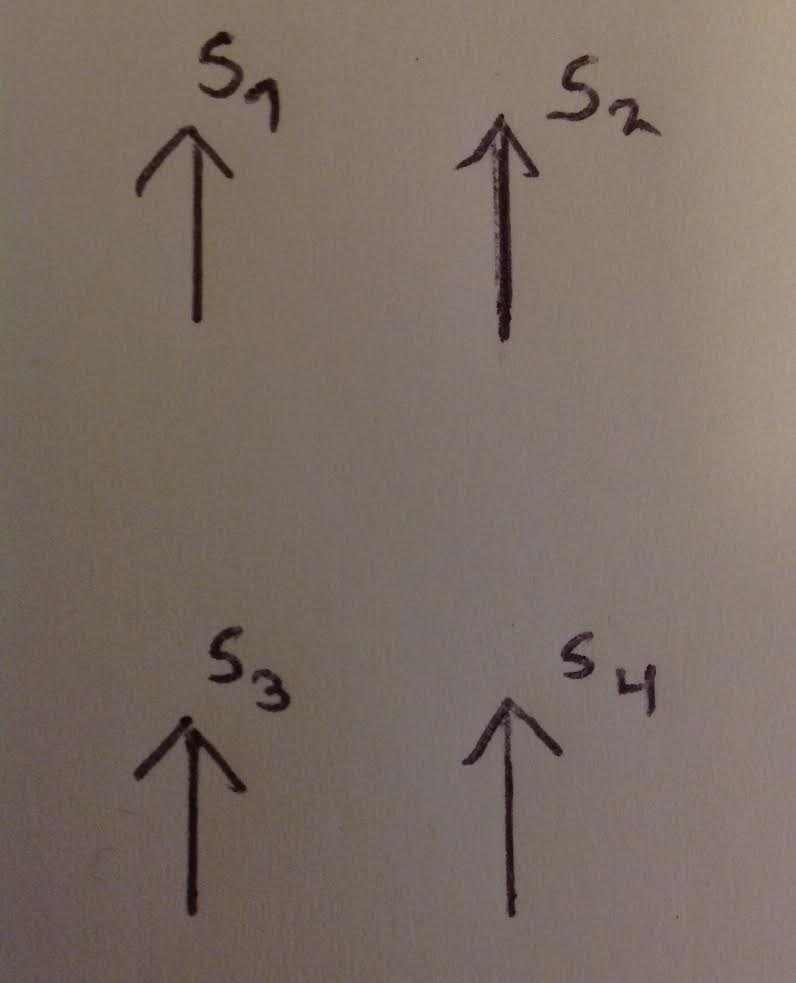
\includegraphics[scale=0.2]{SpinSystem.jpeg}
\caption{One microstate of our $2 \times 2$ lattice, illustrating how we label the spins.}\label{fig:2x2spins}
\end{figure}
\linebreak
We notice first there are only 5 distinct macrostates, namely 0 to 4 spins up. There should be a total of $2^4=16$ microstates. It is clear that the extremes (0 spins up and 4 spins up),  have only one microstate associated with them. The states 1 spin up and 3 spins up each have 4 associated microstates (you can flip one of the four spins). This implies that there are a total of 6 ways to have the state 2 up and 2 down. This is summarized in the table below:\\
\begin{table}[!hb]
\centering
\caption{Number of microstates in a simple $2 \times 2$ lattice}
\begin{tabular}{|c|c|}
\hline
Spins up & Number of microstates\\
\hline
4 & 1\\
3 & 4\\
2 & 6\\
1 & 4\\
0 & 1\\
\hline
\end{tabular}
\end{table}
\linebreak
Now we must investigate the energy of each of these states. In general, the energy with periodic boundary condition for a $2\times 2$ lattice can be written as:
$$E=-J\left[s_1s_2+s_2s_1+s_1s_3+s_3s_1+s_2s_4+s_4s_2+s_3s_4+s_4s_3\right]$$
From this it follows immediately that the energy for the states for 4 spins up or 4 spins down is $-8J$. If we flip one spin, we will flip the sign of exactly half the terms (because each spin occurs in four of the eight pairs). Thus the energy will be zero. If we flip two spins, we can either flip spins that are nearest neighbors (such as $s_1$ and $s_2$, $s_1$ and $s_3$, $s_2$ and $s_4$ or $s_3$ and $s_4$), or we can flip spins that are not nearest neighbors (such as $s_1$ and $s_4$ or $s_2$ and $s_3$). In the first case, we flip the sign of four of the terms in the sum (namely all those that contain one of the two  spins we flip). Thus the total energy will be zero. In the other case, we flip the sign of all terms. Thus the total energy will be 8J.\\
\linebreak
To find the magnetization, we must simply sum the total number of spin up and subtract the number of spin down. This is all summarized in the table below:\\
\begin{table}[!ht]
\centering
\caption{Tallying up important thermodynamical indicators in the simple $2 \times 2$ lattice.}
\begin{tabular}{|c|c|c|c|}
\hline
Spins up &  Energy & Magnetization &Number of microstates\\
\hline
4 &-8J&4&1\\
3 &0 & 2 & 4\\
2 &0 &0 & 4\\
2 & 8J & 0 &2\\
1 &0&-2 & 4\\
0 & -8J & -4& 1\\
\hline
\end{tabular}
\end{table}
\linebreak
This enables us to calculate the partition function as:
$$Z=\sum_{i=1}^{16} e^{-\beta E_i}$$
Where $\beta=1/kT$. As most of the energies are zero, this is relatively straightforward and gives:
$$Z=2e^{8\beta J}+2e^{-8\beta J} + 12=4\cosh (8J\beta) +12$$
We can now compute the expected value of the energy as:
\begin{equation}\label{eq:2x2energy}
\langle E \rangle =  -\frac{\partial \ln Z}{\beta}=-\frac{\partial}{\partial \beta}\ln\left(2e^{8\beta J}+2e^{-8\beta J}+12\right)=\frac{-16Je^{8\beta J}+16Je^{-8\beta J}}{2e^{8\beta J}+2e^{-8\beta J}+12}=-\frac{8J\sinh(8\beta J)}{\cosh(8\beta J)+3}
\end{equation}
Similarly, we can compute the heat capacity, $C_V$, as:
$$C_V=\frac{d\langle E \rangle}{dT}=\frac{d}{dT}\left(\frac{-16Je^{\frac{8J}{kT}}+16Je^{-\frac{8J}{kT}}}{2e^{\frac{8J}{kT}}+2e^{-\frac{8J}{kT}}+12}\right)$$
However, this is an ugly differentiation. Therefore, we will instead use the relation:
$$C_V=\frac{\langle E^2 \rangle - \langle E \rangle^2}{kT^2}$$
The square of the expected value of the energy is given by:
$$\langle E^2\rangle=\frac{1}{Z} \sum_{i=1}^ {16}E_i^2e^{-\beta E_i}$$
The sum is easy to compute:
$$\sum_{i=1}^{16}E_i^2e^{-\beta E_i}=64J^2e^{8J\beta}+128J^2e^{-8J\beta}+64J^2e^{8J\beta}=128J^2\left(e^{8J\beta}+e^{-8J\beta}\right)$$
Which gives:
$$\langle E^2\rangle = \frac{128J^2\left(e^{8J\beta}+e^{-8J\beta}\right)}{2e^{8J\beta}+2e^{-8J\beta}+12}=\frac{256J^2\cosh(8J\beta)}{4\cosh(8J\beta)+12}$$
From which it follows that:
$$C_V=\frac{1}{kT^2}\left(\frac{128J^2\left(e^{8J\beta}+e^{-8J\beta}\right)}{2e^{8J\beta}+2e^{-8J\beta}+12}-\left(\frac{-16Je^{8\beta J}+16Je^{-8\beta J}}{2e^{8\beta J}+2e^{-8\beta J}+12}\right)^2\right)$$

\begin{equation}\label{eq:2x2Cv}
C_V=\frac{1}{kT}\left(\frac{256J^2\cosh(8J\beta)}{4\cosh(8J\beta)+12}-\left(\frac{-8J\sinh(8J\beta)}{\cosh(8J\beta)+3}\right)^2\right)
\end{equation}

Magnetization can be computed as:
$$\langle M \rangle=\frac{1}{Z}\sum_{i=1}^{16}M_ie^{-\beta E_i}$$
The sum can be computed as:
$$\sum_{i=1}^{16}M_ie^{-\beta E_i}=4e^{8J\beta}+8-8-4e^{8J\beta}=0$$
Thus the expected value of the magnetization is zero. The expected value of the absolute value of the magnetization on the other hand is:
\begin{equation}\label{eq:2x2abs_mag}
\langle |M|\rangle =\frac{1}{Z}\sum_{i=1}^{16}|M_i|e^{-\beta E_i}=\frac{1}{Z}\left( 4e^{8J\beta}+4\cdot 2+ 4\cdot 2 +4e^{8J\beta}\right)=\frac{2e^{8J\beta}+4}{\cosh(8J\beta)+3}
\end{equation}
The square of expected value of the magnetization can be computed as:
$$\langle M^2 \rangle = \frac{1}{Z}\sum_{i=1}^{16}M_i^2e^{-\beta E_i}=\frac{1}{Z}\left(16e^{8\beta J}+4\cdot 4+4\cdot 4+16e^{8\beta J}\right)=\frac{8e^{8\beta J}+8}{\cosh(8J\beta)+3}$$
Now it is easy to compute the susceptibility:
\begin{equation}\label{eq:2x2Sus}
\chi = \frac{\langle M^2\rangle - \langle M \rangle^2}{kT}=\frac{1}{kT}\left(\frac{8e^{8\beta J}+8}{\cosh(8\beta J)+3}\right)
\end{equation}
We can now simulate a $2\times 2$ lattice, and check if equations \ref{eq:2x2energy}, \ref{eq:2x2Cv}, \ref{eq:2x2abs_mag} and \ref{eq:2x2Sus} hold true, which gives us a consistency check for our methods.
\newpage
\section{Methods}
\subsection{Energy in our system}\label{energy_in_system}
Note that the sum in equation \ref{eq:ising_system_energy} is only over the nearest neighbors. Therefore, the change in energy from the flip of a single spin (as in the Metropolis algorithm), depends only on the configuration of the nearest neighbors (which are only four spins). This means that there are only a limited number of possible energy differences, $\Delta E$. As shown here \cite{Metropolis}, the only possible values of $\Delta E$ are:
$$\Delta E = \{ -8J, -4J, 0, 4J, 8J\}$$
Wen can therefore precompute the Boltzmann factor, $e^{-\beta \Delta E}$, for all of these possible flips. Thus, for each spin flip in the Metropolis algorithm, we can simply check the configuration of the neighboring spins, and then assign an energy change, $\Delta E$, by checking the state of the neighboring spins, as described in more detail in section \ref{metropolis_algo_implementation}.\\
\linebreak
Not that this works well for all but the initial configuration. For the initial configuration, we will have to compute the total energy. This can be done by a nested for-loop construction, where we always include the energy from the spin above and to the left of our current spin, to avoid double counting. This is shown in the pseudo code below:
\lstinputlisting{Pseudo_code_total_energy.cpp}
\subsection{Implementing periodic boundary conditions}
The periodic boundary conditions can be implemented by using modular division. Each spin will have four nearest neighbors in the lattice. Assume our selected spin is at $x_i$, $y_i$. This spin will be affected by the spin at position $x_{i+1}$, $y_i$ and $x_{i-1}$, $y_i$ (as well as the corresponding spins in the y-idrection). If $x_i$ is on the boundary of our lattice, however, the point to the left or to the right may not exist. Therefore, we find adjacent points by using the following formula:
\begin{equation}\label{eq:modular_arithmetic}
x_{i+1}=(x_{i+1}+N) \bmod N
\end{equation}
Note that, if $x_{i+1}$ happens to element number $N$, this equation gives element 0, and if $x{i-1}$ happens to be element 0, the equation gives element number $N-1$. Thus, this implements the periodic boundary conditions.
\subsection{Implementing the Metropolis algorithm}\label{metropolis_algo_implementation}
The Metropolis algorithm is also implemented as two nested for-loops: the outer one, where we sum over Monte Carlo steps, and the inner one where we sum over $N\times N$ randomly selected spins.\\
\linebreak
As we mentioned in section \ref{energy_in_system}, we can precompute all possible energy differences. Thus, when we propose a spin flip, we must simply compute the energy change due to the flip, which can be found from:
$$\Delta E = 2J\sum_k s_is_k$$
Where the sum extends over all neighbors of the spin $s_i$. We can then associate this $\Delta E$ with the correct, precomputed, Boltzmann factor, and do the comparison described in section \ref{Monte-Carlo_algo}.  This is shown in Pseudo-code below. Note that we here disregard the periodic boundary conditions, for improved readability. 
\lstinputlisting{Pseudo_code_Metropolis.cpp}
\subsection{Investigating the time taken to arrive at the most likely state and the underlying probability distribution}
We wish to investigate how the equilibration time (time to reach most likely state) of our system depends on the temperature of our system, and on the initial configuration. We adapt a plain graphical approach - we simply plot the time development of the mean energy and the mean absolute value of the magnetization, to find when the (initially large) deviations die out. An alternative way to characterize equilibrium is, as discussed in section \ref{equilibrium_system}, with the total number of accepted configurations. Therefore, we include a plot of this as well.\\
\linebreak
Additionally, we would also like to characterize the probability distribution governing the equilibrium state. Therefore, we start our simulation after the time which we determined to be the equilibration time, and compute the number of times a given energy $E$ appears.
\subsection{Investigating phase transitions}
To investigate the phase transitions that occur in the Ising system, we employ the fact that the analytic result for $T_C(N=\infty)$ from section \ref{phase_tranisition} is approximately 2.269, as stated here \cite{Project}. Thus we choose temperatures close to this, and find the critical temperature (the temperature at which a divergent behavior is observed for the heat capacity and the magnetic susceptibility). Then we compare with the equations from section \ref{phase_tranisition}.
\subsection{Parallelizing our code}
Note that the quantities that we are investigating are statistical measures such as the expected value or the variance. Increasing the number of cycles will therefore result in a better data. To maximize the number of cycles that we can obtain we parallelize our code, using MPI. Thus, we let all four cores on our computer run separate simulations, and then compute the means using the data from all of these runs.\footnote{Note that we initially intended to run on a larger cluster but, due to time constraints, this was not possible.}
\newpage
\section{Results}
In this section, we present the results from our investigation. We postpone an extended discussion of these results until the next section.
\subsection{Results from the 2 $\times$ 2 lattice}
We begin by investigating the number of steps required to get a good correspondence between the analytic expressions from section \ref{2x2analytic} and our simulations. We choose to compare the heat capacity of the system, as this has the most complex form. We let each core run an $N$ that is divisible by $10$, so that the total number of steps will be $4$ times a number divisible by $10$. Note that we plot all of these quantities \textit{per spin} to ease readability.\\
\begin{figure}[!ht]
    \centering
    \begin{subfigure}[H!]{0.5\textwidth}
        \centering
        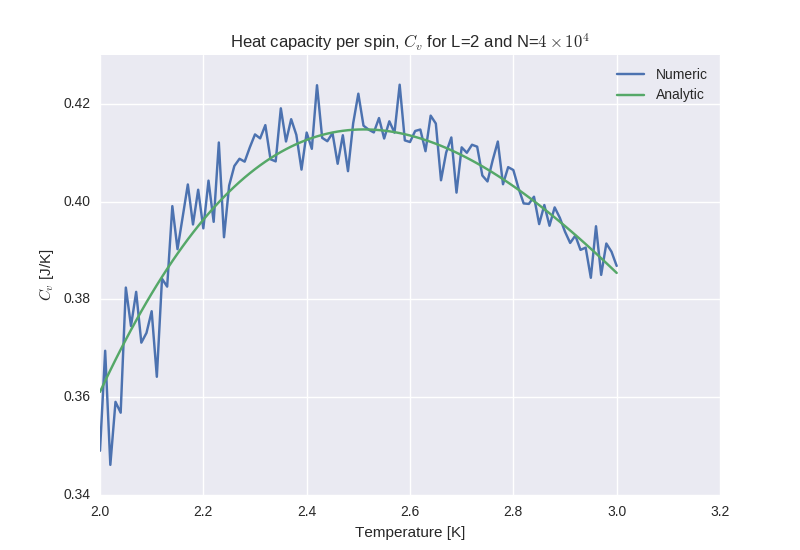
\includegraphics[height=2.2in]{L2Cv4e4.png}
        \caption{$N=4\times 10^4$}
    \end{subfigure}%
    ~ 
    \begin{subfigure}[H!]{0.5\textwidth}
        \centering
        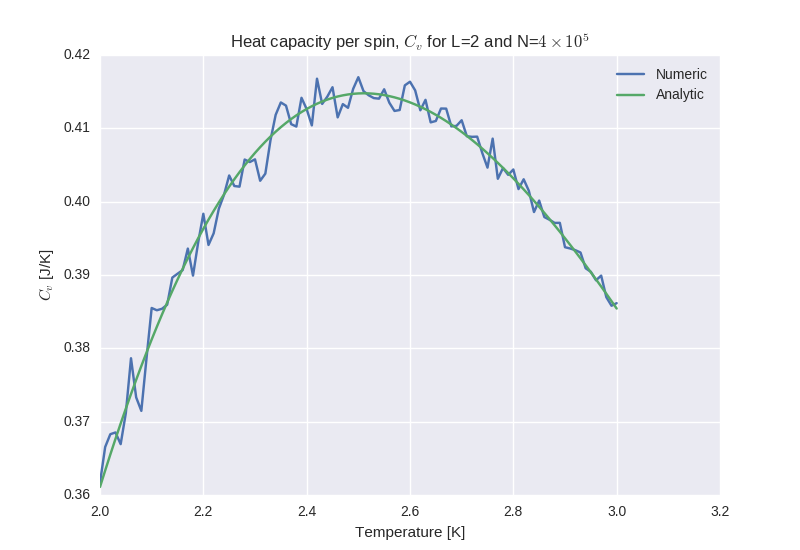
\includegraphics[height=2.2in]{L2Cv4e5.png}
        \caption{$N=4\times 10^5$}
    \end{subfigure}
    \begin{subfigure}[H!]{0.5\textwidth}
        \centering
        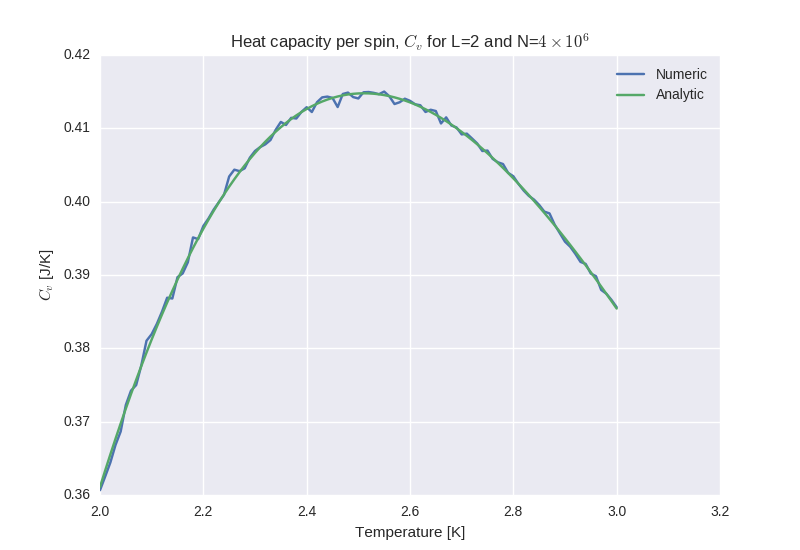
\includegraphics[height=2.2in]{L2Cv4e6.png}
        \caption{$N=4\times 10^6$}
    \end{subfigure}%
    ~ 
    \begin{subfigure}[H!]{0.5\textwidth}
        \centering
        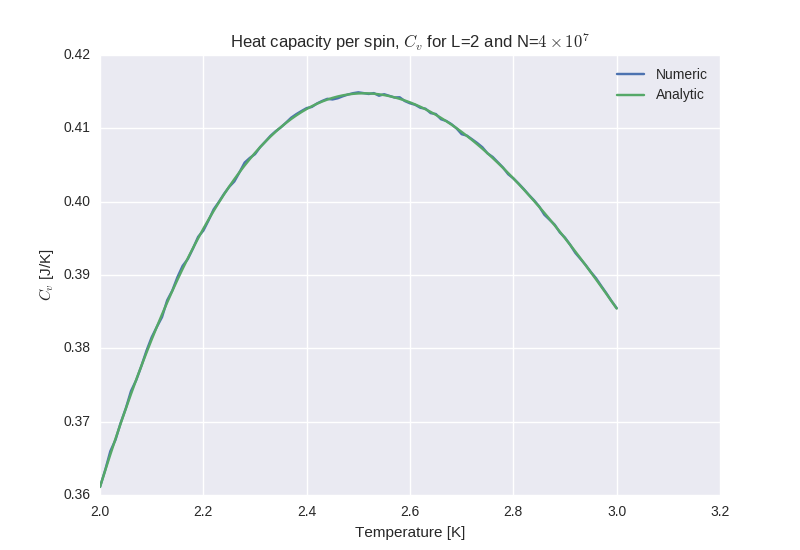
\includegraphics[height=2.2in]{L2Cv4e7.png}
        \caption{$N=4\times 10^7$}
    \end{subfigure}
    \caption{Comparison of the numeric and analytic solution of heat capacity and mean energy per spin for the $2\times 2$ lattice. We plot multiple Monte Carlo steps, $N$, to find where the correspondence becomes good. This was done with temperatures in the interval $kT/J=2$ to $kT/J=3$.}\label{fig:2x2_nsteps}
\end{figure}
\linebreak
We also compare explicitly the value from the Ising model and the analytic solution at $kT/J=1$ in table \ref{tab:2x2_compare} below.
\newpage
\begin{table}[!ht]
\centering
\caption{Explicit comparison for the $2 \times 2$ lattice at the point $kT/J=1$ for different Monte Carlo cycles, $N$.}\label{tab:2x2_compare}
\begin{tabular}{|c|ccccc|}
\hline
$N$ & $4 \times 10^4$ & $4\times 10^5$ & $4\times 10^6$ & $4 \times 10^7$ & Analytic\\ 
\hline
$ \langle E \rangle [J]$ &  -1.9961 & -1.9962 & -1.9961 & -1.9960 & -1.9960\\
$\langle |M|\rangle $ [J/T] &3.9946 &  3.9946 &3.9948 & 3.9946 & 3.9946\\
$C_v$ [J/K] &0.0315 & 0.0305 & 0.0311 & 0.0321 & 0.0320 \\
$\chi$ [J $\mathrm{s}^2$] &3.950 & 3.991 & 3.984 & 3.993 & 3.993 \\
\hline
\end{tabular}
\end{table}

Looking at the plots, we choose $N=4\times 10^7$ as the required $N$, as this gives an excellent correspondence between the analytic and the numeric solution. The plots of our thermodynamic quantities in the $2\times 2$ lattice for this value of $N$ are shown below:
\begin{figure}[!ht]
    \centering
    \begin{subfigure}[H!]{0.5\textwidth}
        \centering
        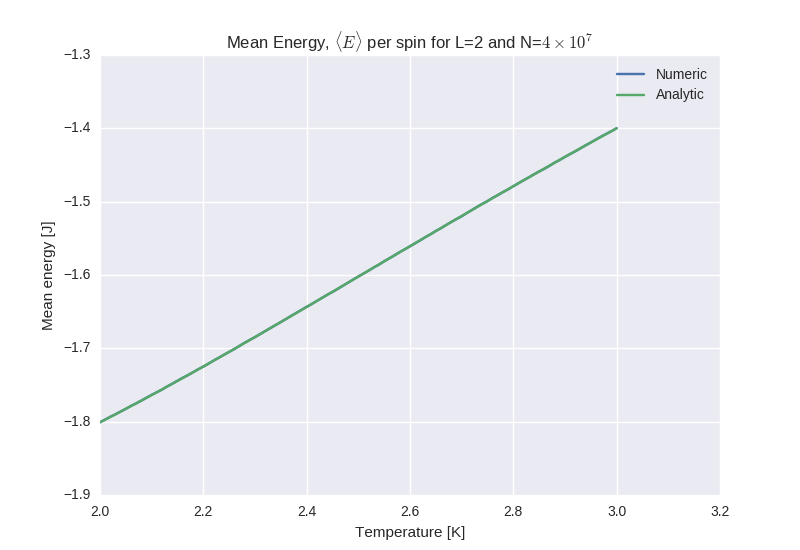
\includegraphics[height=2.2in]{L2MeanEner4e7.png}
        \caption{Mean energy per spin}
    \end{subfigure}%
    ~ 
    \begin{subfigure}[H!]{0.5\textwidth}
        \centering
        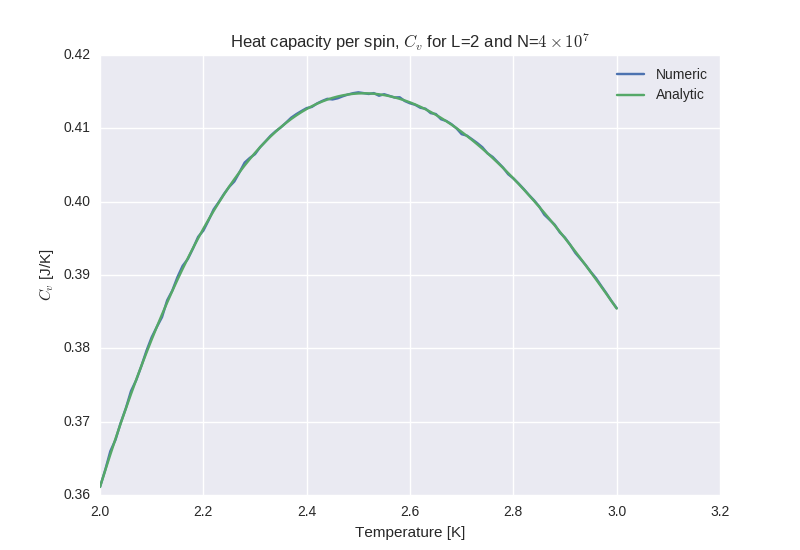
\includegraphics[height=2.2in]{L2Cv4e7.png}
        \caption{Heat capacity per spin}
    \end{subfigure}
    ~
     \begin{subfigure}[H!]{0.5\textwidth}
        \centering
        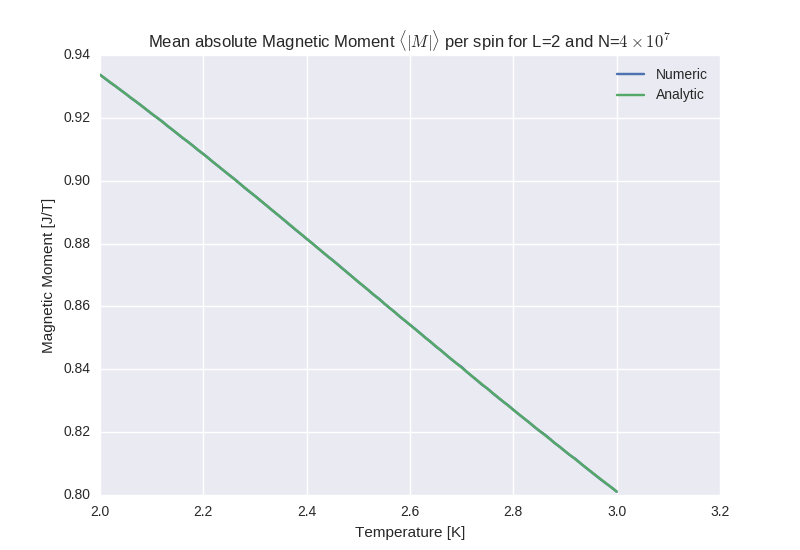
\includegraphics[height=2.2in]{L2MeanabsMag4e7.png}
        \caption{Mean absolute magnetic moment per spin}
    \end{subfigure}%
    ~ 
    \begin{subfigure}[H!]{0.5\textwidth}
        \centering
        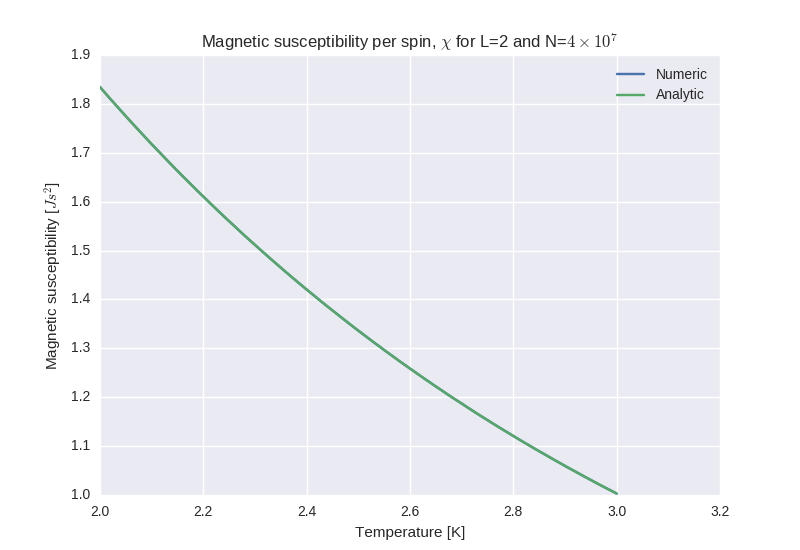
\includegraphics[height=2.2in]{L2MagSus4e7.png}
        \caption{Magnetic susceptibility per spin}
    \end{subfigure}
    \caption{Comparison of the numeric and  analytic solution for the mean energy per spin, heat capacity per spin, mean absolute magnetic moment per spin and magnetic susceptibility of the $2 \times 2$ lattice, running $10^7$ Monte Carlo cycles for each temperature. }\label{fig:2x2_thermo}
\end{figure}
\newpage
\subsection{Results from our investigation into the time used to reach equilibrium for larger system}
We choose to use a larger lattice, of $20 \times 20$ spins, to investigate the time (measured in number of sweeps of the lattice) that it takes our system to achieve equilibrium. We investigate this first with a low temperature (letting $kT/J=1.0$). We look at how this system develops if we start with an ordered initial state (all spins pointing up) and if we start with a disordered (uniformly distributed) state. A plot of the mean energy and the mean absolute value of the magnetization in this case is shown below:\\
\begin{figure}[!ht]
    \centering
    \begin{subfigure}[H!]{0.5\textwidth}
        \centering
        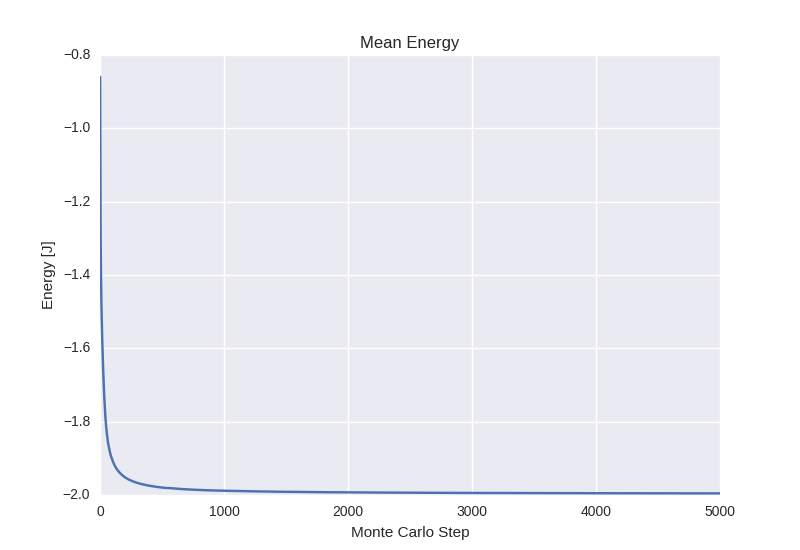
\includegraphics[height=2.2in]{meanEnergyWRandomStart.png}
        \caption{Mean energy per spin from disordered state}
    \end{subfigure}%
    ~ 
    \begin{subfigure}[H!]{0.5\textwidth}
        \centering
        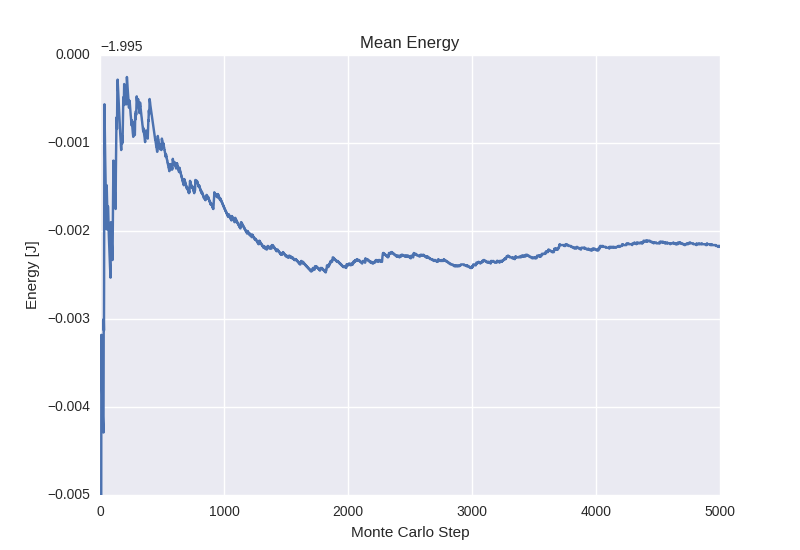
\includegraphics[height=2.2in]{meanEnergyWUpStart.png}
        \caption{Mean energy per spin from uniform state}
    \end{subfigure}
        ~
     \begin{subfigure}[H!]{0.5\textwidth}
        \centering
        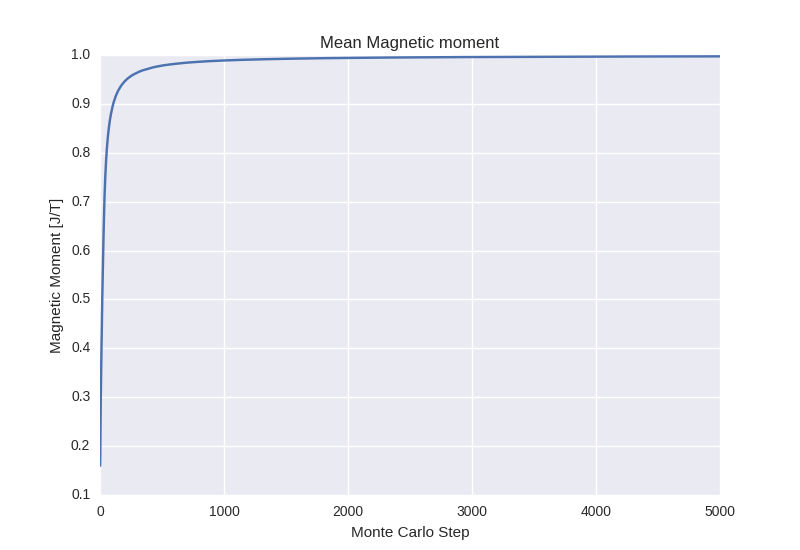
\includegraphics[height=2.2in]{meanMagMomWRandomStart.png}
        \caption{Mean absolute magnetic moment per spin from disordered state}
    \end{subfigure}%
    ~ 
    \begin{subfigure}[H!]{0.5\textwidth}
        \centering
        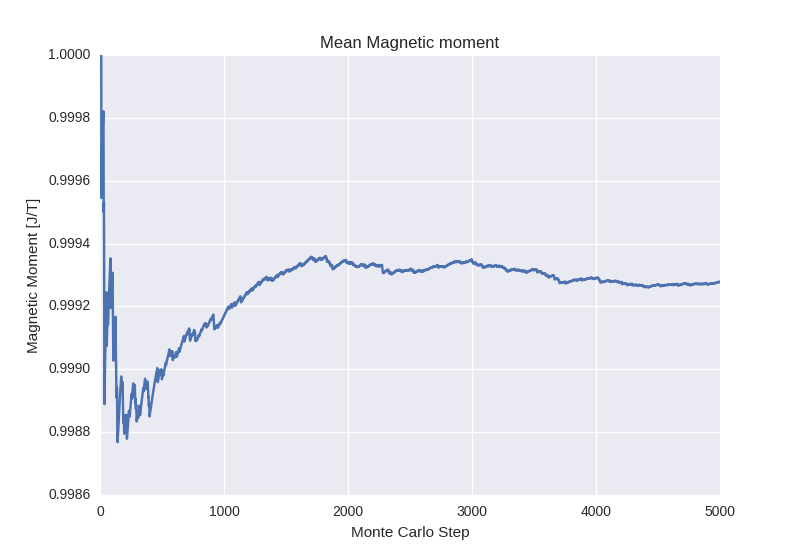
\includegraphics[height=2.2in]{meanMagMomWUpStart.png}
        \caption{Mean absolute magnetic moment per spin from uniform state}
    \end{subfigure}
      \caption{Time development of mean energy and mean magic moment per spin for two different initial configurations.Here $L=20$ and $kT/J=1.0$.}\label{fig:20x20_Sweep_T_1}
\end{figure}
\linebreak
We also plot the same quantities for a temperature of $kT/J=2.4$ in the figure below:
\newpage
\clearpage
\begin{figure}[!ht]
    \centering
    \begin{subfigure}[H!]{0.5\textwidth}
        \centering
        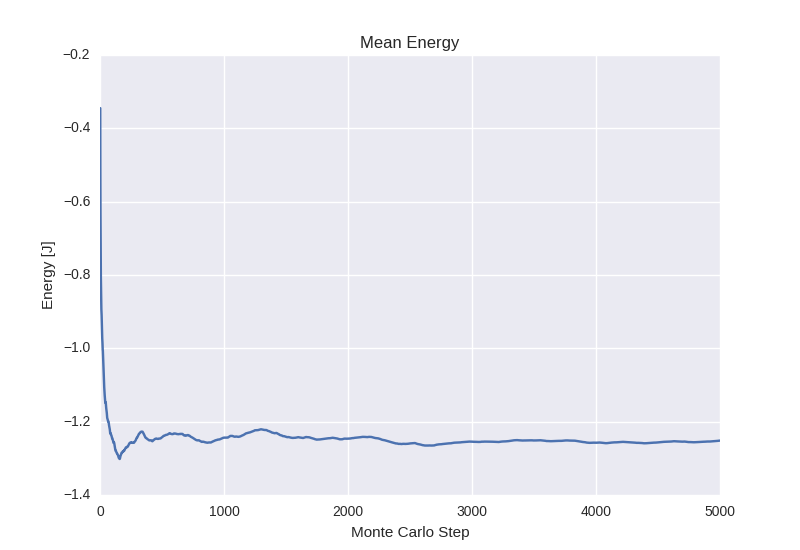
\includegraphics[height=2.2in]{meanEnergyWRandomStartT24.png}
        \caption{Mean energy per spin from disordered state}
    \end{subfigure}%
    ~ 
    \begin{subfigure}[H!]{0.5\textwidth}
        \centering
        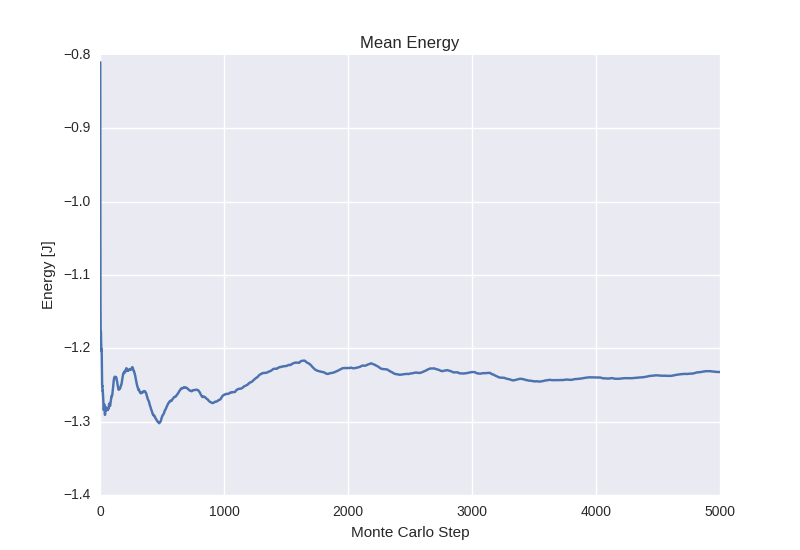
\includegraphics[height=2.2in]{meanEnergyWUpStartT24.png}
        \caption{Mean energy per spin from uniform state}
    \end{subfigure}
        ~
     \begin{subfigure}[H!]{0.5\textwidth}
        \centering
        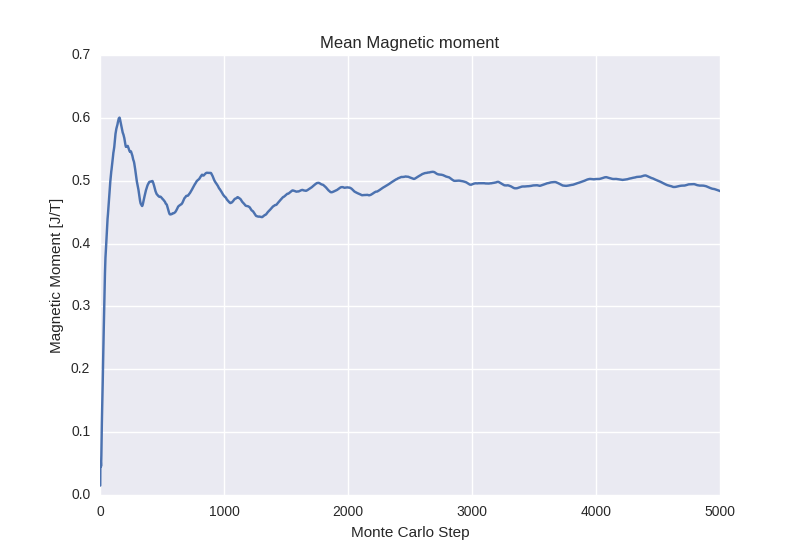
\includegraphics[height=2.2in]{meanMagMomWRandomStartT24.png}
        \caption{Mean absolute magnetic moment per spin from disordered state}
    \end{subfigure}%
    ~ 
    \begin{subfigure}[H!]{0.5\textwidth}
        \centering
        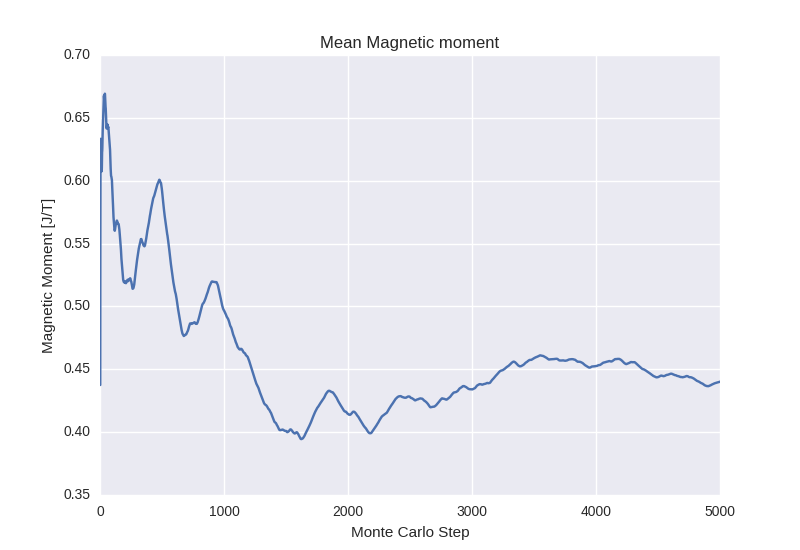
\includegraphics[height=2.2in]{meanMagMomWUpStartT24.png}
        \caption{Mean absolute magnetic moment per spin from uniform state}
    \end{subfigure}
      \caption{Time development of mean energy and mean magic moment per spin for two different initial configurations. Here $L=20$ and $kT/J=2.4$.}\label{fig:20x20_Sweep_T_24}
\end{figure}

Finally, we also plot the number of accepted flips per spin and time, to get a sense of how many spins the Metropolis algorithm flips at every time step. We do this for two different temperatures, again using both an ordered and a disordered state.
\clearpage
\begin{figure}[!ht]
    \centering
    \begin{subfigure}[H!]{0.5\textwidth}
        \centering
        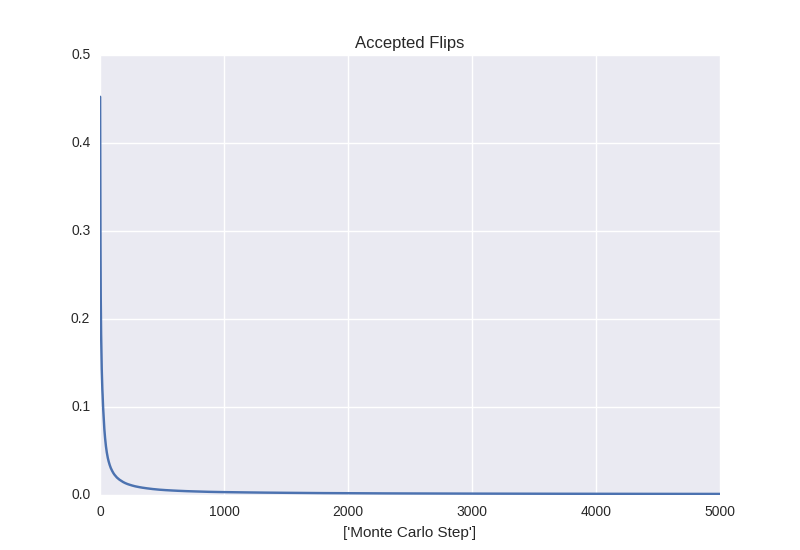
\includegraphics[height=2.2in]{flipsWRandomStart.png}
        \caption{With disordered initial state, at $kT/J=1$}
    \end{subfigure}%
    ~ 
    \begin{subfigure}[H!]{0.5\textwidth}
        \centering
        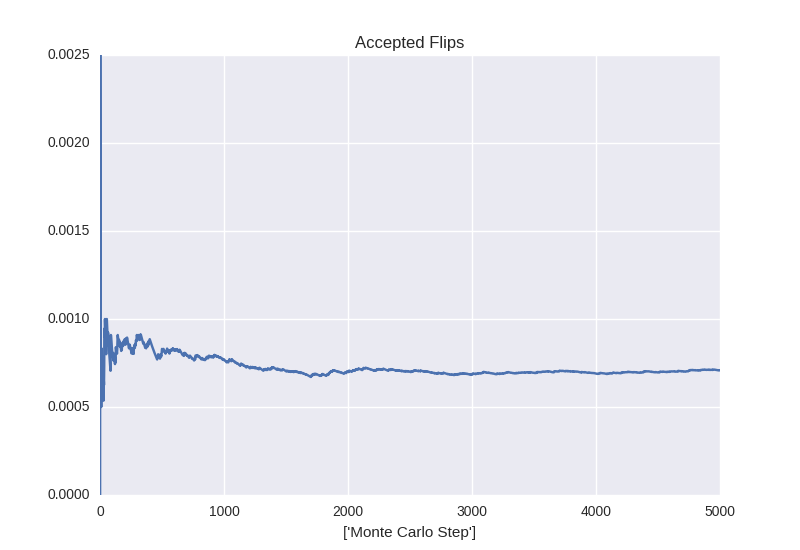
\includegraphics[height=2.2in]{flipsWUpStart.png}
        \caption{With uniform initial state, at $kT/J=1$}
    \end{subfigure}
        ~
     \begin{subfigure}[H!]{0.5\textwidth}
        \centering
        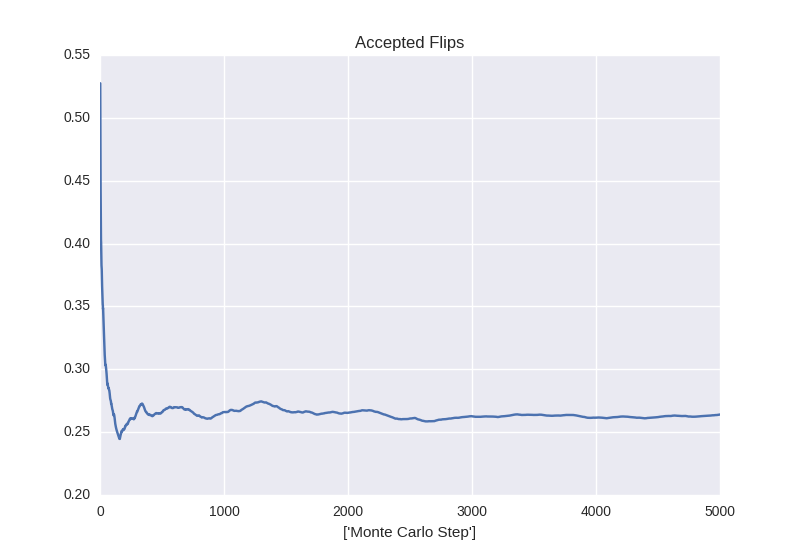
\includegraphics[height=2.2in]{flipsWRandomStartT24.png}
        \caption{With disordered initial state, at $kT/J=2.4$}
    \end{subfigure}%
    ~ 
    \begin{subfigure}[H!]{0.5\textwidth}
        \centering
        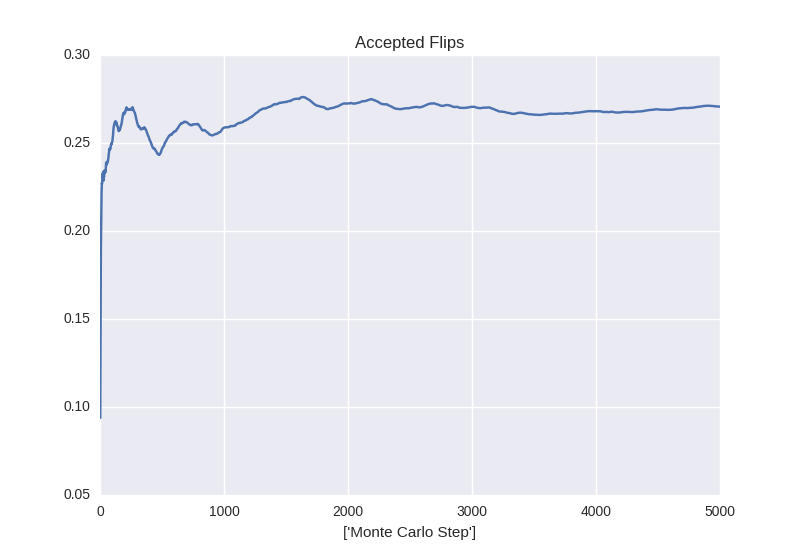
\includegraphics[height=2.2in]{flipsWUpStartT24.png}
        \caption{With uniform initial state, at $kT/J=2.4$}
    \end{subfigure}
      \caption{Mean number of accepted flips per spin per Monte Carlo cycle for different initial states and different temperatures.}\label{fig:20x20_Sweep_flips}
\end{figure}
All these figures seem to indicate that equilibrium is quickly reached (after less than 2000 cycles). However, sometimes this is not the case, as we hit a local minimum (described in more detail in section \ref{Discussion_time_for_eq}). This gives the following plots:
\clearpage
\begin{figure}[!ht]
    \centering
    \begin{subfigure}[H!]{0.5\textwidth}
        \centering
        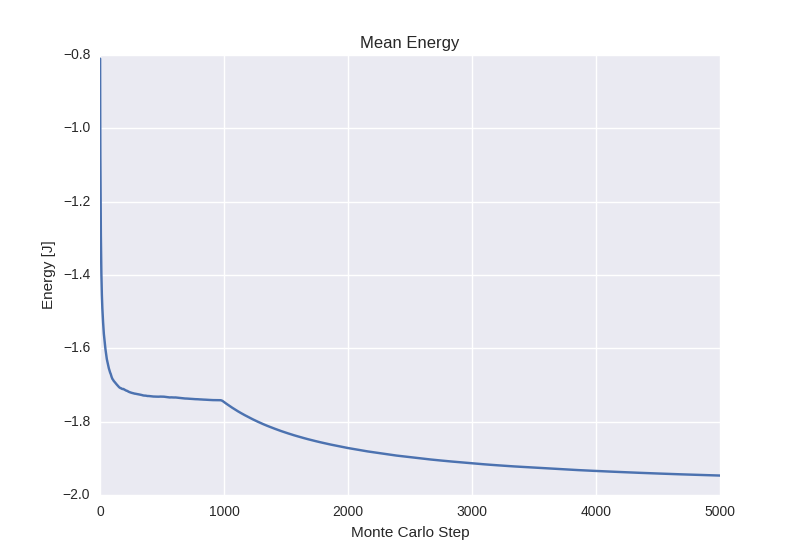
\includegraphics[height=2.2in]{meanEnergyLocalMin.png}
        \caption{Mean energy per spin from uniform state}
    \end{subfigure}%
    ~ 
    \begin{subfigure}[H!]{0.5\textwidth}
        \centering
        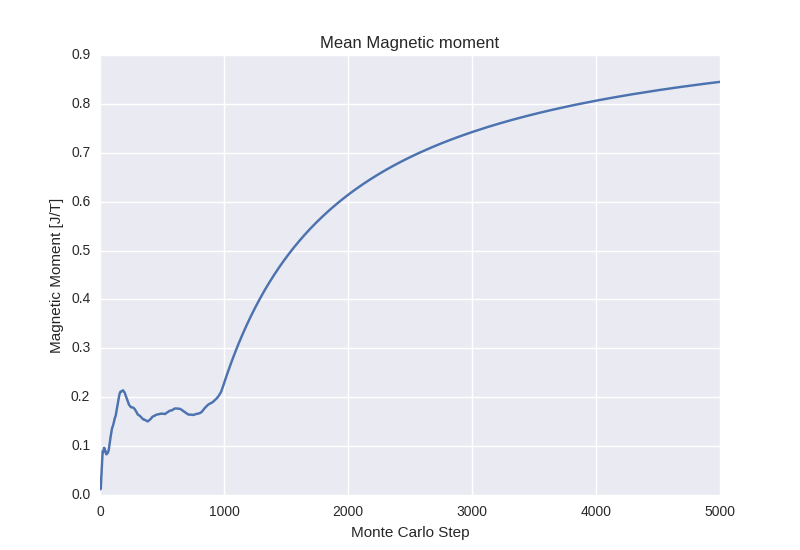
\includegraphics[height=2.2in]{meanMagMomLocalMin.png}
        \caption{Mean magnetic moment per spin from uniform state}
    \end{subfigure}
     ~ 
    \begin{subfigure}[H!]{0.5\textwidth}
        \centering
        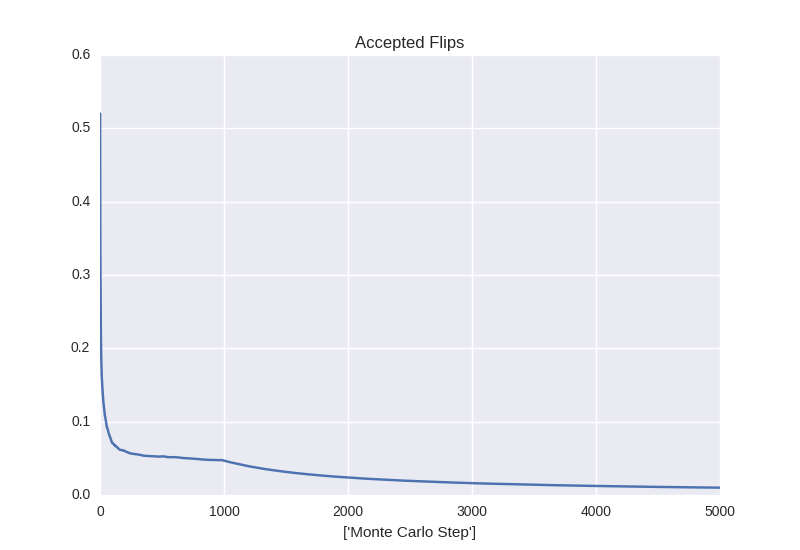
\includegraphics[height=2.2in]{flipsLocalMin.png}
        \caption{Mean number of accepted flips per spin per Monte Carlo cycle from uniform state}
    \end{subfigure}
       \caption{Time development of mean energy, mean magnetic moment and mean number of accepted flips per spin per Monte Carlo cycle for a system with $L=20$, $kT/J=1$, with all spins initially pointing up.}\label{fig:20x20_local_min}
\end{figure}
This shows that it sometimes takes significantly longer to arrive at equilibrium. Furthermore, equilibration time may also increase for higher temperature. Therefore, we choose 5000 Monte Carlo cycles as a safe equilibration time.
\newpage
\subsection{Results from our investigation into the probability distribution}
Here we plot the probability of a certain energy occurring for two different temperatures.
\begin{figure}[!ht]
    \centering
    \begin{subfigure}[H!]{0.5\textwidth}
        \centering
        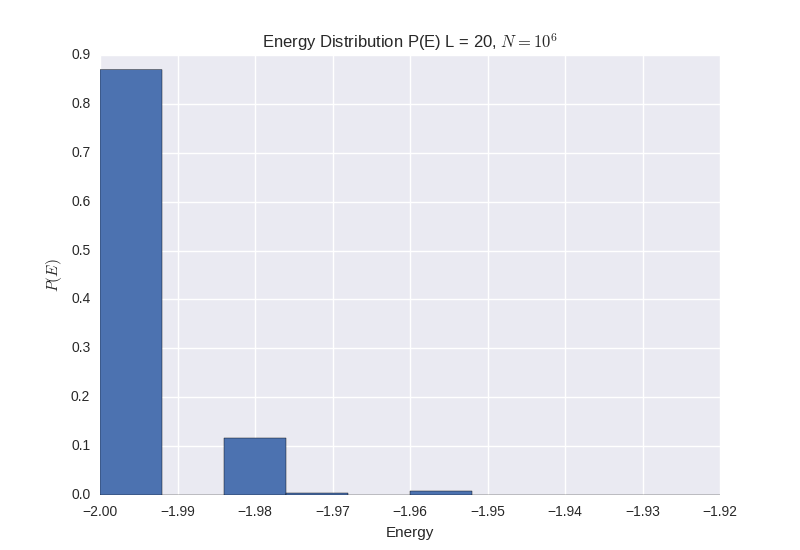
\includegraphics[height=2.2in]{energyDistHistoT1.png}
        \caption{$kT/J=1$}
    \end{subfigure}%
    ~ 
    \begin{subfigure}[H!]{0.5\textwidth}
        \centering
        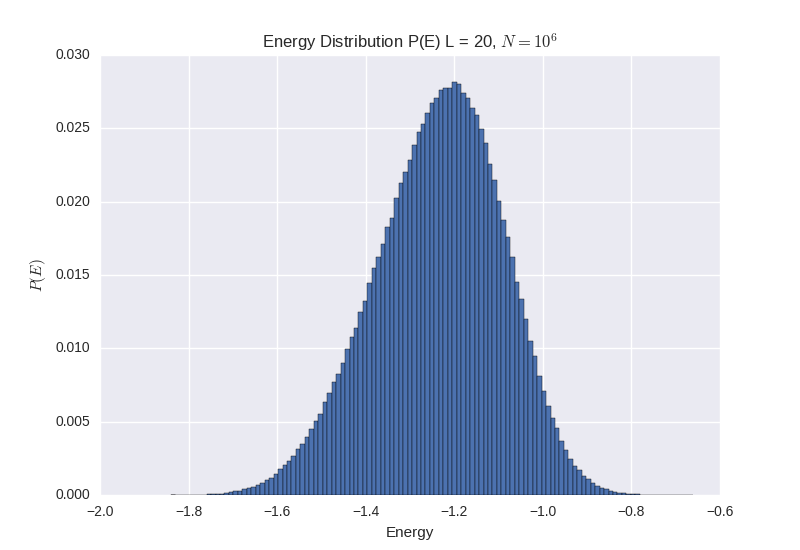
\includegraphics[height=2.2in]{energyDistHisto.png}
        \caption{$kT/J=2.4$}
    \end{subfigure}
       \caption{Histogram showing the probability of different energies occurring for two different temperature. This is for a lattice with $L=20$, simulated with $N=10^5$ Monte Carlo cycles, excluding an equilibration time of 5000 cycles. }\label{fig:histograms}
\end{figure}

\subsection{Results from our investigation of phase transitions}
Here, we wish to investigate how the critical temperature, which we extract by looking at the susceptibility and heat capacity, depends on our lattice size $L$. We also include the mean energy and the absolute value of the mean magnetization for completeness. We will discuss the number of temperature points that we chose in greater detail in section \ref{discussion_phase_transition}.\\
\clearpage
\begin{figure}[!ht]
    \centering
    \begin{subfigure}[H!]{0.5\textwidth}
        \centering
        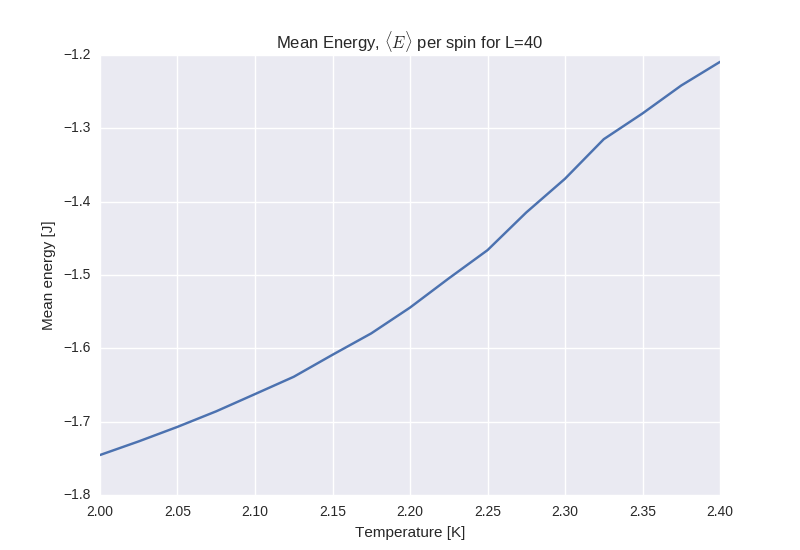
\includegraphics[height=2.2in]{meanEnergyl40Ne5New.png}
        \caption{Mean energy per spin for $L=40$}
    \end{subfigure}%
    ~ 
    \begin{subfigure}[H!]{0.5\textwidth}
        \centering
        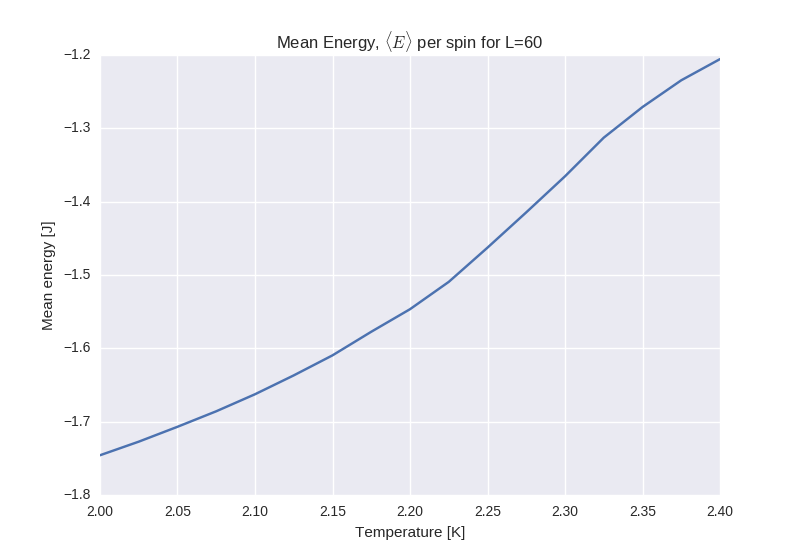
\includegraphics[height=2.2in]{meanEnergyl60Ne5New.png}
        \caption{Mean energy per spin for $L=60$}
    \end{subfigure}
        ~
     \begin{subfigure}[H!]{0.5\textwidth}
        \centering
        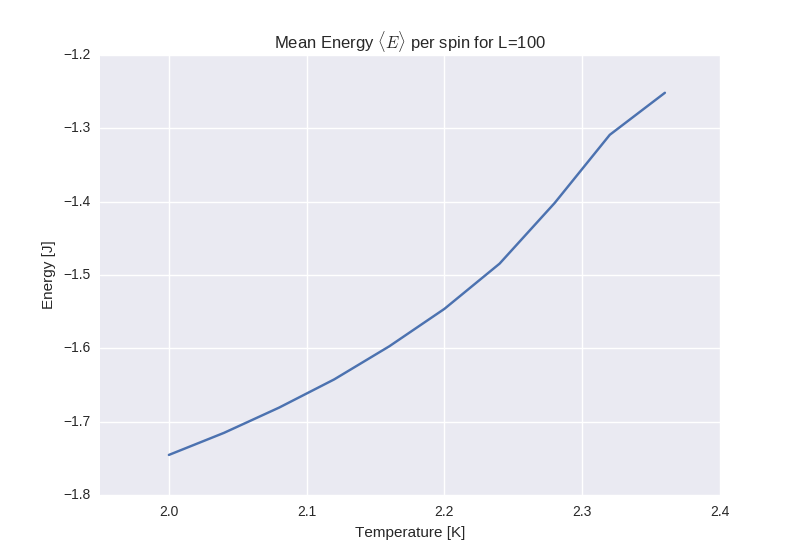
\includegraphics[height=2.2in]{meanEnergyl100Ne5New.png}
        \caption{Mean energy per spin for $L=100$}
    \end{subfigure}%
    ~ 
    \begin{subfigure}[H!]{0.5\textwidth}
        \centering
        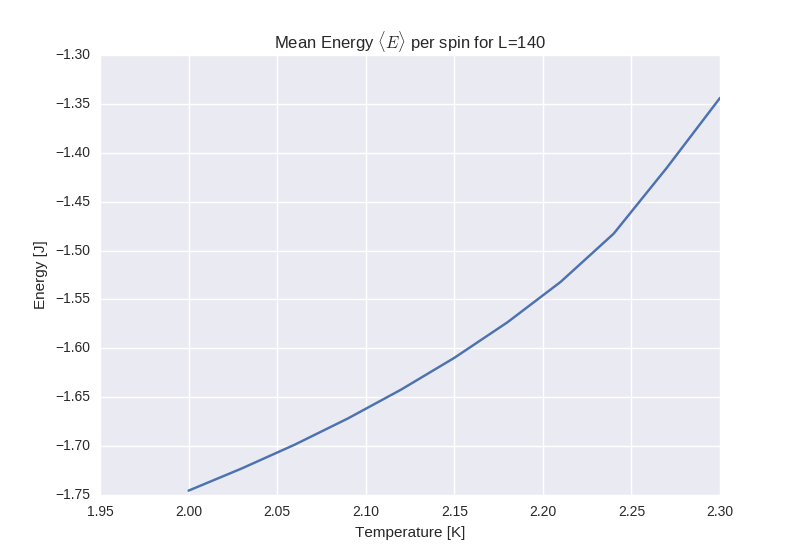
\includegraphics[height=2.2in]{meanEnergyl140.png}
        \caption{Mean energy per spin for $L=140$}
    \end{subfigure}
      \caption{Development of the mean energy per spin for systems of different sizes, as a function of temperature. We simulated $10^5$ Monte Carlo cycles, excluding an equilibration time of 5000 cycles.}\label{fig:phase_tranition_energy}
\end{figure}
\clearpage
\begin{figure}[!ht]
    \centering
    \begin{subfigure}[H!]{0.5\textwidth}
        \centering
        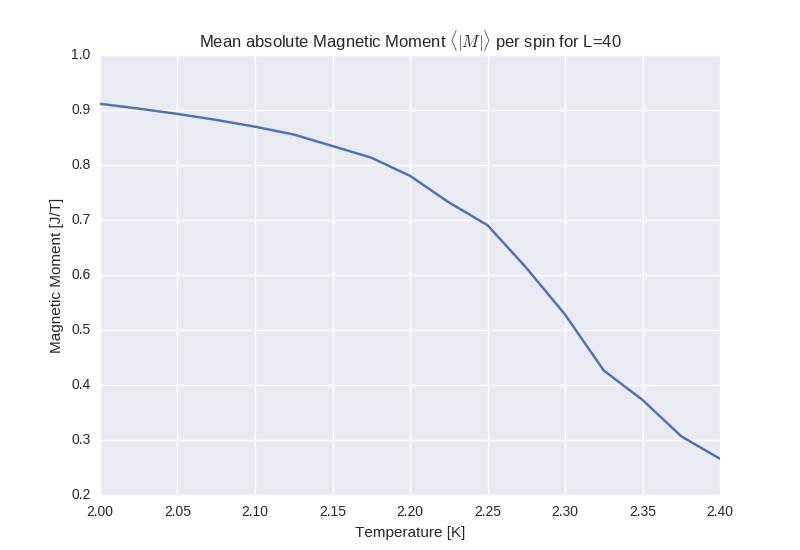
\includegraphics[height=2.2in]{meanMagMoml40Ne5New.png}
        \caption{Mean absolute value of the magnetic moment per spin for $L=40$}
    \end{subfigure}%
    ~ 
    \begin{subfigure}[H!]{0.5\textwidth}
        \centering
        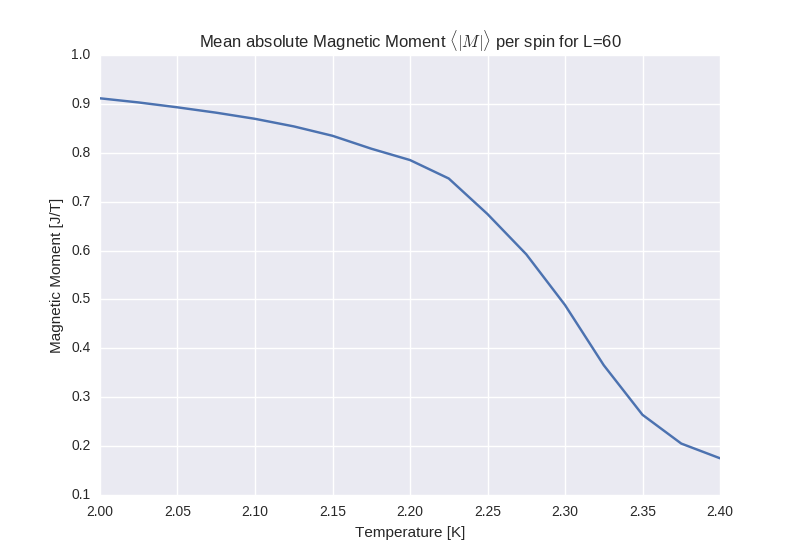
\includegraphics[height=2.2in]{meanMagMoml60Ne5New.png}
        \caption{Mean absolute value of the magnetic moment per spin for $L=60$}
    \end{subfigure}
        ~
     \begin{subfigure}[H!]{0.5\textwidth}
        \centering
        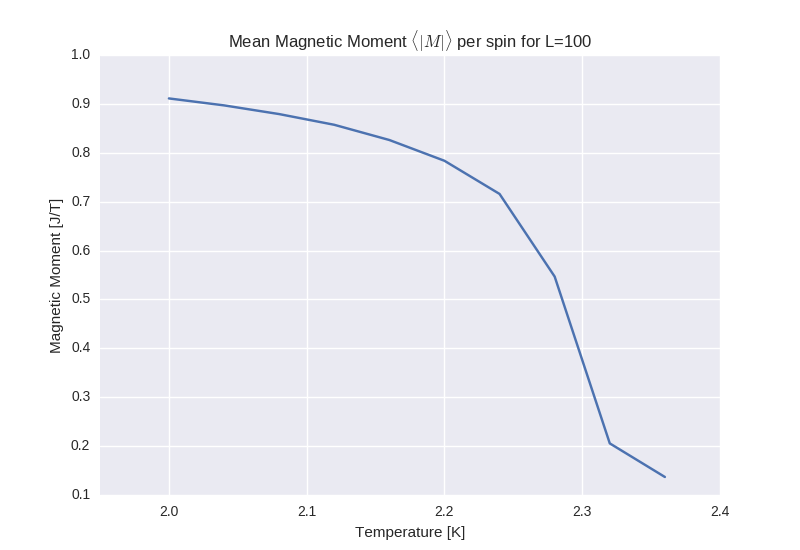
\includegraphics[height=2.2in]{meanMagMoml100Ne5New.png}
        \caption{Mean absolute value of the magnetic moment per spin for $L=100$}
    \end{subfigure}%
    ~ 
    \begin{subfigure}[H!]{0.5\textwidth}
        \centering
        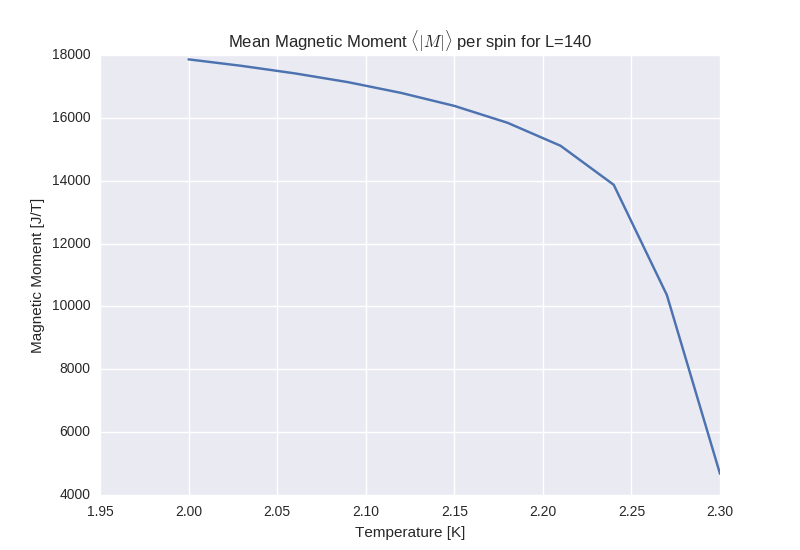
\includegraphics[height=2.2in]{meanMagMoml140.png}
        \caption{Mean absolute value of the magnetic moment per spin for $L=140$}
    \end{subfigure}
      \caption{Development of the mean absolute value of the magnetic moment per spin for systems of different sizes, as a function of temperature. We simulated $10^5$ Monte Carlo cycles, excluding an equilibration time of 5000 cycles.}\label{fig:phase_mag_mom}
\end{figure}
\clearpage
\begin{figure}[!ht]
    \centering
    \begin{subfigure}[H!]{0.5\textwidth}
        \centering
        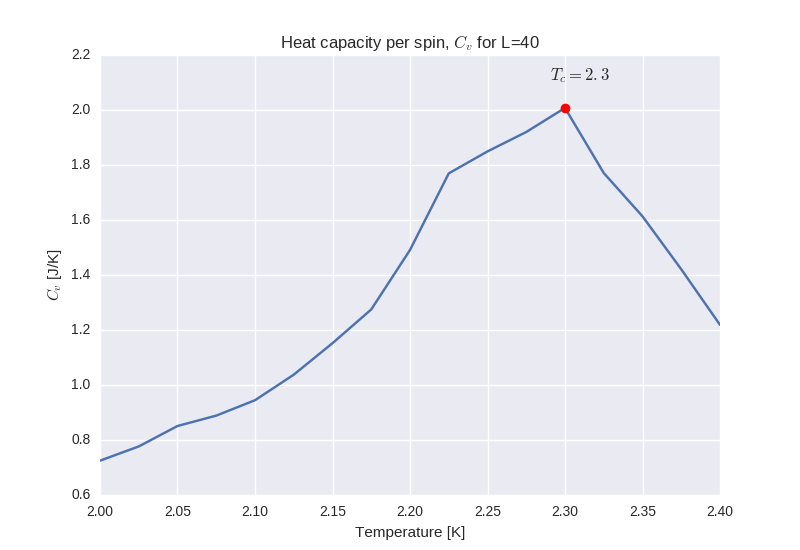
\includegraphics[height=2.2in]{cvl40Ne5New.png}
        \caption{Heat capacity for $L=40$}
    \end{subfigure}%
    ~ 
    \begin{subfigure}[H!]{0.5\textwidth}
        \centering
        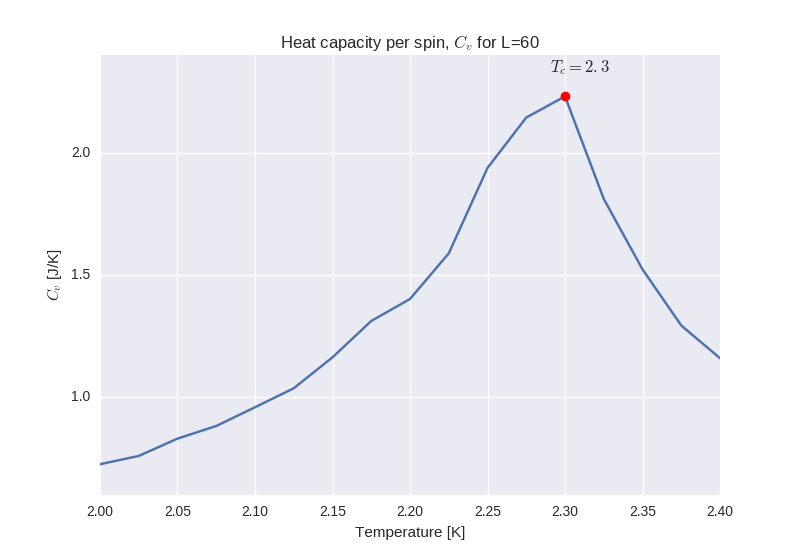
\includegraphics[height=2.2in]{cvl60Ne5New.png}
        \caption{Heat capacity for $L=60$}
    \end{subfigure}
        ~
     \begin{subfigure}[H!]{0.5\textwidth}
        \centering
        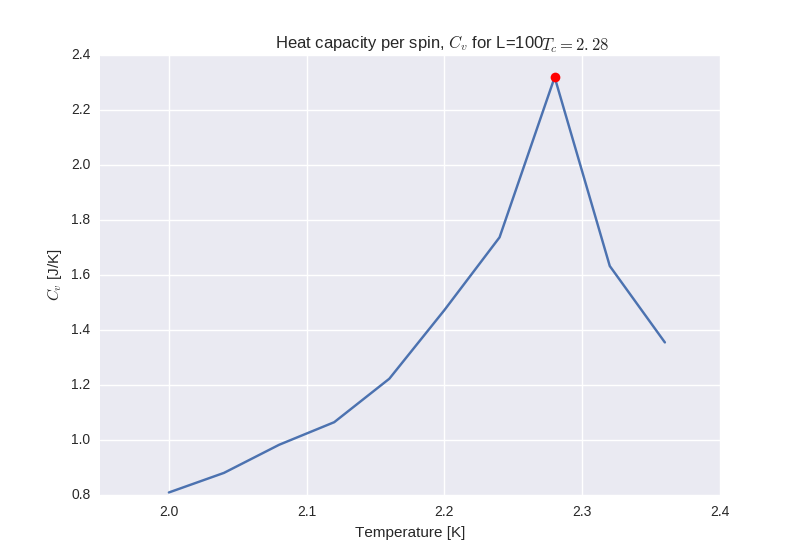
\includegraphics[height=2.2in]{cvl100Ne5New.png}
        \caption{Heat capacity for $L=100$}
    \end{subfigure}%
    ~ 
    \begin{subfigure}[H!]{0.5\textwidth}
        \centering
        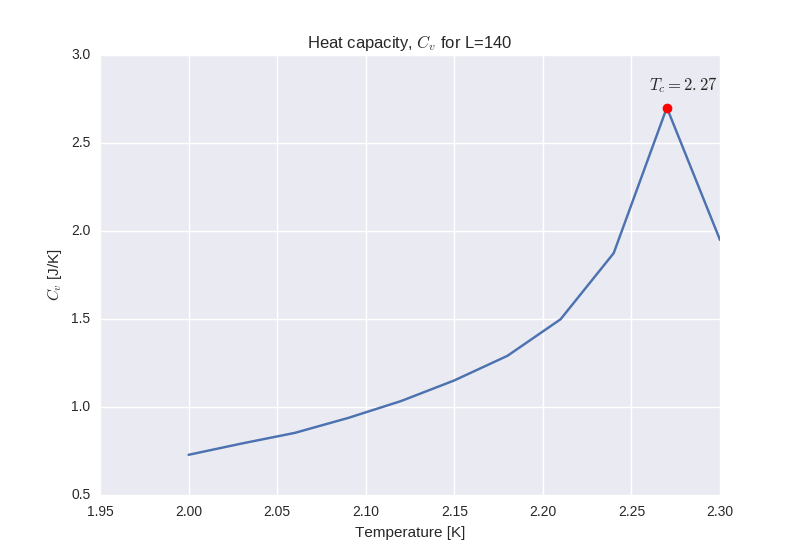
\includegraphics[height=2.2in]{cvl140.png}
        \caption{Heat capacity for $L=140$}
    \end{subfigure}
      \caption{Development of the heat capacity for systems of different sizes, as a function of temperature. We simulated $10^5$ Monte Carlo cycles, excluding an equilibration time of 5000 cycles.}\label{fig:phase_Cv}
\end{figure}
\clearpage
\begin{figure}[!ht]
    \centering
    \begin{subfigure}[H!]{0.5\textwidth}
        \centering
        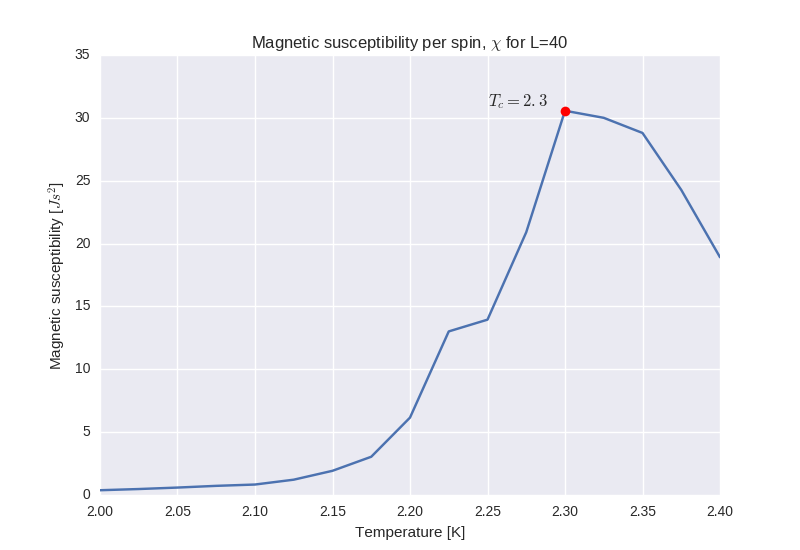
\includegraphics[height=2.2in]{chil40Ne5New.png}
        \caption{Magnetic susceptibility for $L=40$}
    \end{subfigure}%
    ~ 
    \begin{subfigure}[H!]{0.5\textwidth}
        \centering
        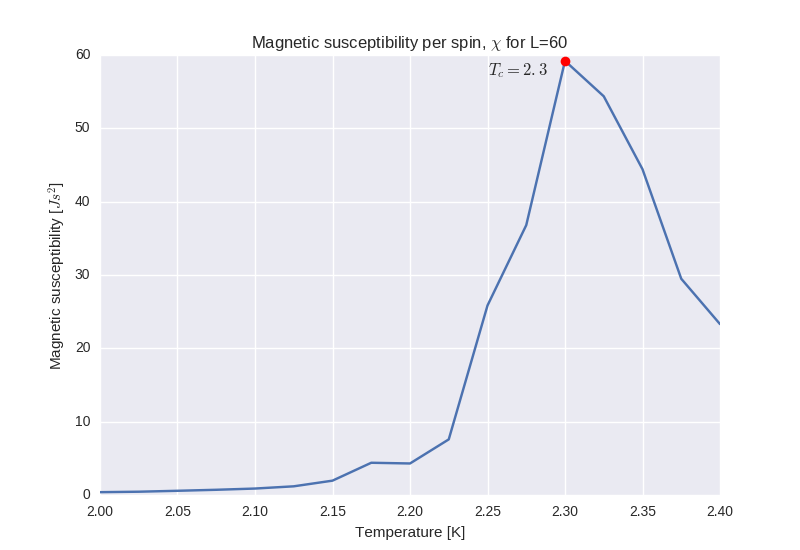
\includegraphics[height=2.2in]{chil60Ne5New.png}
        \caption{Magnetic susceptibility for $L=60$}
    \end{subfigure}
        ~
     \begin{subfigure}[H!]{0.5\textwidth}
        \centering
        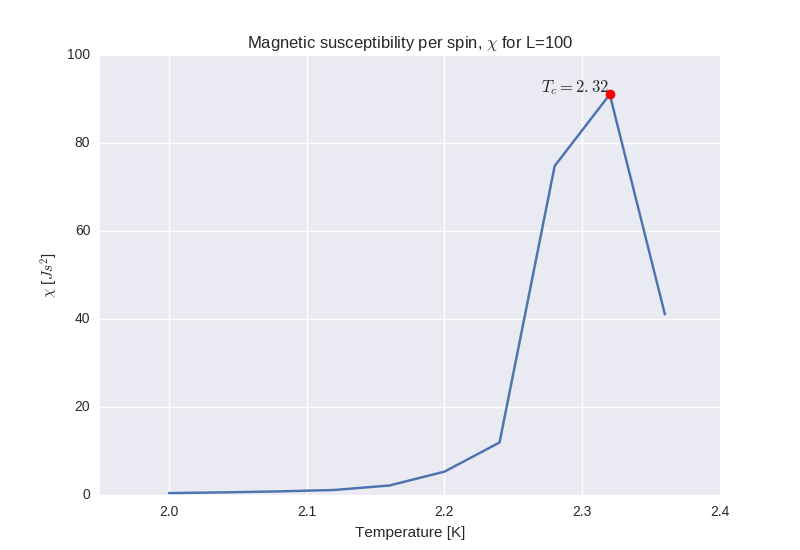
\includegraphics[height=2.2in]{chil100Ne5New.png}
        \caption{Magnetic susceptibility for $L=100$}
    \end{subfigure}%
    ~ 
    \begin{subfigure}[H!]{0.5\textwidth}
        \centering
        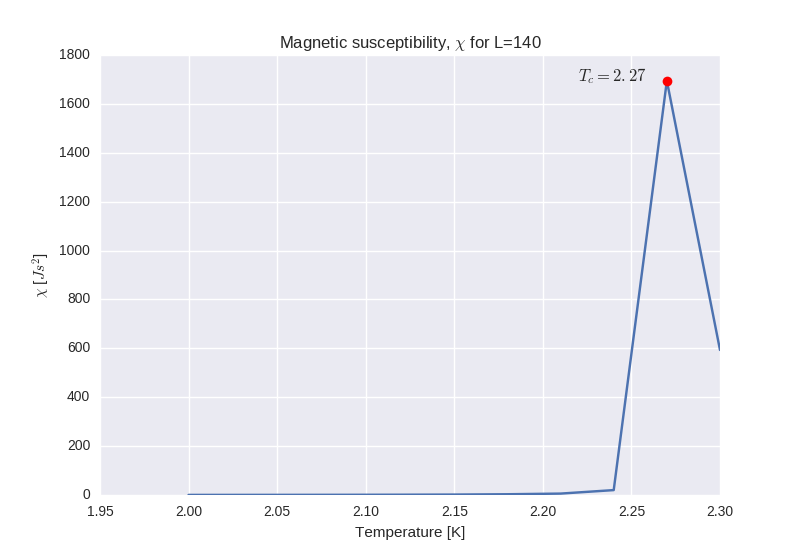
\includegraphics[height=2.2in]{chil140.png}
        \caption{Magnetic susceptibility for $L=140$}
    \end{subfigure}
      \caption{Development of the magnetic susceptibility for systems of different sizes, as a function of temperature. We simulated $10^5$ Monte Carlo cycles, excluding an equilibration time of 5000 cycles.}\label{fig:phase_chi}
\end{figure}
\subsection{Results from parallelizing our code}
\begin{table}[!ht]
\centering
\caption{Comparison of speed with and without parallelization for a $20 \times 20$ lattice. We compare for numbers of Monte-Carlo cycles, $N$.}\label{tab:compare_parallelized}
\begin{tabular}{|c|c|c|}
\hline
N & With MPI [s] &  Without MPI [s]\\
\hline
\rule{0pt}{2ex}    
$4\cdot 10^5$ & 4.08 & 11.296 \\
$4 \cdot 10^6$ & 45.347 & 109.675\\ 
\hline
\end{tabular}
\end{table}
\clearpage
\section{Discussion}
\subsection{The 2 $\times$ 2 lattice}
Figure \ref{fig:2x2_nsteps} compares the analytic and numeric solution for a different number of Monte Carlo cycles. As expected, our numeric solution approaches the analytic solution with increasing $N$, and for $N=4\times 10^7$, the solutions are barely distinguishable. Notice also how almost all quantities shown in table \ref{tab:2x2_compare} correspond to the exact quantities, at least to the precision shown. Though the table shows some random fluctuations for the earlier values of $N$, these seem to have died out in this case. Therefore, we adapt $10^7$ as an acceptable $N$, for this system.  Note further that, with this $N$,all other thermodynamic quantities shown in figure \ref{fig:2x2_thermo} are also very well reproduced by our code. This shows that our simulations converge to the expected values for the $2\times2$ lattice, which hopefully implies that our code also works for larger lattices, for which there are no analytic solutions. The error is truly small at $N=10^7$, which therefore seems to be an ideal number of cycles to perform. Note, however, that $N=10^7$ was not attainable for our later, larger, simulations within our strict time constraints. Therefore, we performed the remaining simulations with $N=10^5$ instead, but started our data collection after a certain equilibration time has passed, as will be explored in detail in the next section. Note that this means the system does not have to "balance out" the large errors in the means that are incurred by starting far away from the equilibrium state. Therefore, the hope is that we will be able attain useful data even with less cycles.
\subsection{Time required to reach equilibrium}\label{Discussion_time_for_eq}
Figure \ref{fig:20x20_Sweep_T_1} and \ref{fig:20x20_Sweep_T_24} show the time development of our system for different temperatures. Note that uniform initial state here refers to a configuration where all spins are initially pointing upwards, whereas disordered initial state refers to a configuration where the spin is drawn from a uniform distribution containing only the values -1 and +1.\\
\linebreak
There are several interesting points to note:
\begin{itemize}
\item The spins in the uniform initial state generally start much closer to equilibrium than the spins in the disordered initial state
\item The equilibrium states differs for the different temperatures
\item The start point of the mean absolute magnetic moment per spin for the uniform initial state is not at 1.
\end{itemize}
The first point is not very surprising. Both temperatures are fairly low, and we therefore expect the equilibrium state to be fairly ordered. Therefore, if we start in an ordered state, we will already be much closer to equilibrium. Therefore, it takes less time to achieve equilibrium. \\
\linebreak
The second point is not particularly surprising either. At a higher temperature, we expect there to be more disturbance in the crystal (more thermal motion), so that the equilibrium state will be less uniform. This is indeed what we observe - the equilibrium mean magnetic moment is lower (which corresponds to less spins being aligned) and the mean energy per spin is less negative, from which it follows that the spins are less tightly bound. Thus the Ising model corresponds well with physical intuition. Notice further how the discrepancy between the equilibration time for the uniform initial state and the disordered initial state has decreased. They now both reach equilibrium after approximately 2000 Monte-Carlo cycles, whereas for the case where $kT/J=1$, the uniform state essentially started in the equilibrium configuration (note the scale of the axes!).\\
\linebreak
The final point is slightly more surprising. Given that we start in a uniform state, we would expect the mean absolute magnetic moment per spin to start close to 1, but it clearly does not. One possible explanation is that we hit a relatively Monte-Carlo cycle, where the magnetic moment decreased by a large amount the first iteration (note that we do not write out the initial configuration). This would however indeed be a very unlikely occurrences, so it is an interesting behavior to observe. \\
\linebreak
Figure \ref{fig:20x20_Sweep_flips} shows the mean number of accepted flips per spin per Monte Carlo cycle for varying initial states and temperatures. The trend in these figures is very similar to the trend in the previous figures. At the low-temperature limit, the uniform initial state starts at what is essentially the equilibrium configuration. Therefore, very few flips are accepted. This quickly stabilizes, and the system forgets all about the initial state, stabilizing at a very low average number of flips per spin, per cycle. This makes sense, because the Boltzmann factors are so large in this case, so that the Metropolis algorithm will only very rarely flip a spin. Note that the low-temperature, disordered state takes much longer to reach this equilibrium (has a much higher relaxation time). The reason is that we initially flip a large number of spins, to get into equilibrium, and as we plot the \textit{mean} number of accepted flips, this will increase the mean even long after the flip in every time step has reached equilibrium. Thus, if we measure mean flips, the time for the system to forget its initial state and reach equilibrium is much higher in the disordered initial state.\\
\linebreak
A very similar pattern can be seen for the high temperature, but it is less pronounced, due to the same factors as earlier - we start further from the equilibrium in the uniform case, and closer to equilibrium in the disordered case, then we did at the lower temperature. Thus these two solutions approach each other, and at high temperatures, they would even switch roles. Notice also that the equilibrium line is much higher at the higher temperatures. The Boltzmann factors are smaller, so more flips will be successful in the Metropolis algorithm, even at equilibrium. If one dares to translate this observation into actual physics, it follows that more is happening, at a microscopic level, at higher temperatures - even at equilibrium.\\
\linebreak
Finally, note carefully figure \ref{fig:20x20_local_min}. This is such a striking behavior that we initially thought that we had discovered a bug. In fact, this figure shows a local minimum in the Ising system. Notice that we are at a low temperature, starting from a uniform system. What happens, is that we the Monte Carlo sweep, by chance, manages to select a large number of spins in one region. The result is that these spins will be flipped to align with their neighbors, so that we get different regions in which the spins are aligned with each other (they can be all aligned upwards in some region, all downwards in another region etc.). If we now pick a spin inside any of those regions, it will be fairly stable with respect to its neighbors. Depending on the shape of the regions, it may be rather unlikely to pick a spin on the boundary. Therefore, this transitional  state can persist for some time, until the regions break up, as can be seen - the curves appear to reach an equilibrium without actually being in an equilibrium state. This forces us to reevaluate our equilibration time. From the previous plots,an equilibration time of about 2000 cycles may not seem unreasonable. However, figure \ref{fig:20x20_Sweep_T_1} shows that this would be far too low. Therefore, we decide to let the equilibration time be 5000 cycles. From figure \ref{fig:20x20_local_min}b in particular, this may still seem like a low number. Notice, however, that local minima of the duration shown in \ref{fig:20x20_local_min} are rather rare - we did not observe many of them. Furthermore, as we will be simulating $10^5$ cycles after this equilibration time, a slight, initial, deviation from the equilibrium values will not be crucial for the outcome of our simulations.
\subsection{The probability distribution}
We show in figure \ref{fig:histograms} how the probability distribution for our energies varies with temperature. We do this by simply counting up the number of times the different energies appear, and then divide by the total number of occurrences.\\
\linebreak
In the low temperature state, our space of attained energies is very small. By the ergodic hypothesis, all microstates should be equally likely, so we should be able to span all of them if we simulate long enough. Clearly this has yet to occur here, which demonstrates that the most likely state by far is the leftmost state, at an energy of almost precisely 2.\\
\linebreak
For the high-temperature limit, we observe a qualitatively different behavior. It spans a significantly larger subset of all accessible energies, and has  much higher mean. Both of these make physical sense - at higher temperature, the spins will, as earlier stated, be less tightly bound to their neighbors, and are freer to flip, giving a larger average energy at equilibrium. Additionally, however, the fact that the spins are freer to flip, means that more frequent flips will occur, even at equilibrium, which can take much furhter from equilibrium than in the low-temperature case. It is interesting to observe that the shape seems to approach a Gaussian distribution. This makes some sense: in this regime, above the critical temperature (discussed in section \ref{phase_tranisition}) the flips are governed largely by random fluctuations, as the larges-scale structures somewhat break down. It would be interesting to compare this to the variance of the energy, to see if the variance is much higher - however, this was not possible due to time constraints.
\subsection{The phase transitions}\label{discussion_phase_transition}
Figures \ref{fig:phase_tranition_energy}, \ref{fig:phase_mag_mom}, \ref{fig:phase_Cv} and \ref{fig:phase_chi} show the behavior of our system as a function of temperature. Note, first of all, that the scales on the axis is not quite the same. We began (for $L=40$ and $L=60$), with points in the interval $[2\mathrm{kT/J}, 2.4\mathrm{kT/J}]$, with $0.025 \mathrm{kT/J}$ between each point. However, we realized that the interesting physics (the phase transition) occurred at around $2.3 kT/J$. To save time, we therefore decided to simulate only until $T=2.35 kT/J$, with steps of $0.04$ for the $L=100$ case. After considering the data from $L=100$, we decided that it would be sufficient to simulate $L=140$ up to a temperature of $2.3 kT/J$, with steps of 0.03 $kT/J$. Thus the odd axis are a result of limited computation time.\\
\linebreak
Note furthermore, that we have adapted a slight trick - we use $\langle |M|\rangle$ in the equation for the magnetic susceptibility (equation \ref{eq:magnetic_susp}) instead of $\langle M \rangle$, for all except the $2 \times 2$ lattice. The reason for this is that $\langle M \rangle$ will, for small systems, tend to oscillate significantly, which may result in an error in $\chi$. This disappears if we employ $\langle |M|\rangle$ instead.\\
\linebreak
Note then, in particular figure \ref{fig:phase_Cv} and \ref{fig:phase_chi}, showing respectively the heat capacity and the susceptibility. As mentioned in section \ref{phase_tranisition}, we expect power-laws for $C_v$ and $\chi$. We also expect these macroscopic variables  of our system to change significantly in a phase transition. Therefore, we find the critical temperature at the maximum of the graphs of $C_v$ and $\chi$, which we have indicated by a red dot.\\
\linebreak
Note how both $C_v$ and $\chi$ give the same $T_C$ for all runs, except for $L=100$. Note further, how the values of $T_C$ are all crowded close together around 2.3 $kT/J$. This is problematic, because in order to estimate a correct value for $a$ from equation \ref{eq:a:equation}. However, we do not have a unique value for $T_C$ for $L=100$, and we have identical values for $T_C$ for $L=40$ and $L=60$. We will therefore employ equation \ref{eq:a:equation} with $L_1=60$ and $L_2=140$, as the only viable options. This gives (using the analytic result that $\nu = 1$):
$$a=\frac{2.3-2.27}{60^{-1}-140^{-1}}=3.15$$
Which gives the critical temperature in the thermodynamic limit as (using equation \ref{eq:Critical_temp_at_infinite}):
$$T_C(L=\infty)=T_C(L)-aL^{-1/\nu}=2.27-3.15\cdot 140^{-1}=2.2475$$
The exact analytic expression can be found here \cite{Project}, and is given by:
$$T_C(L=\infty)=\frac{2}{\ln(1+\sqrt{2})}\approx2.269$$
Thus our relative error is $\epsilon_{\mathrm{rel}}\approx 0.95 \%$, which is acceptable, though it is somewhat disappointing that we could only really check this with one point. Notice also that, because the critical temperature was the same for $L=40$, we could have done the same comparison with $L=40$ and $L=140$ (not $L=40$ and $L=60$, as this would give $a=0$). Doing this gives:
$$a=1.68, \quad T_C(L=\infty)=2.258, \quad \epsilon_{\mathrm{rel}}\approx 0.48 \%$$
Thus this would decrease our error. However, as earlier pointed out, it seems odd that the critical temperature should be the same for both cases.
\subsection{The parallelization of our code}
We show in table \ref{tab:compare_parallelized} the difference in speed for a system with $L=40$ of using 4 cores and not using 4 cores. Notice that the difference is large - a significant speed-up was achieved with MPI. This illustrates the fact that parallelization, when it is as straightforward as it is here, can incur huge benefits to the speed of a program.
\clearpage
\section{Conclusion}
\subsection{Conclusion}
We have presented an investigation into various aspects of the Ising model, and how it can be used to model magnetism. We started by comparing our results to a $2\times 2$ lattice, for which we had derived analytic results. We found an excellent correspondence between these models. Then we moved on to larger systems, without analytic solutions, to investigate equilibration time in our model. Here, we found that the equilibration time is generally quite low (dependent on initial configuration and temperature), however, sometimes local minima can occur, which force us to use a larger equilibration time. We also investigated the probability distribution governing our system, and found good correspondence with our physical intuition. Finally, we investigated phase transitions, where we found good correspondence with analytic results, but also clearly saw that additional computational power\footnote{Such as through the cluster Smaug, which we, due to time constraints, were unable to use}, yielding additional grid points for the temperature would have been useful to get a more reliable estimate of the critical temperature.
\subsection{Outlook}
There is still a significant amount of work to do. Most notably: find a better estimate for the critical temperature. Additionally, it would be interesting to investigate the variance of the energy, to see if we manage to achieve some level of correspondence with our distribution. Finally, it may be of interest to further investigate the phase transitions we observed, to study such things as how stable they are, or how many different regions are present in the material.
\addcontentsline{toc}{section}{References}
\bibliography{Project4}
\bibliographystyle{plain}
\newpage
\end{document}